%----------------------------------------------------------------------------------------
% PACKAGES AND OTHER DOCUMENT CONFIGURATIONS
% WARNING: Don't mess with any of the following unless you know what you are doing.
%----------------------------------------------------------------------------------------
\documentclass[english,12pt,a4paper,openany]{book}
\usepackage{datetime}
\usepackage{tabularx}
\usepackage{makecell}
\usepackage{eurosym}
\usepackage{pbox}
\usepackage[utf8]{inputenc}
\usepackage[T1]{fontenc}
\usepackage[english]{babel}
\usepackage{amsmath}
\usepackage{amsfonts}
\usepackage{fancyhdr}
\usepackage{amssymb}
\usepackage[dvipsnames]{xcolor}
\usepackage{mdframed}
\usepackage{multirow}
\usepackage{multicol} 
\usepackage{tikz}
\usepackage{graphicx}
\usepackage[absolute]{textpos} 
\usepackage{colortbl}
\usepackage{array}
\usepackage{geometry}
\usepackage{hyperref}
\pagestyle{fancy}
\renewcommand\headrulewidth{1pt}
\usepackage{float}

%------------------------------------------------------------------------------------------------------
%	The following are the RGB values for the official ATU colours.
%------------------------------------------------------------------------------------------------------	
\definecolor{ATUGreen}{RGB}{0, 91, 94}
\definecolor{ATULightGreen}{RGB}{172, 245, 189}
\definecolor{ATUNavy}{RGB}{0, 26, 121}
\definecolor{ATUOrange}{RGB}{255, 121, 30}
\definecolor{ATUPurple}{RGB}{77, 8, 87}
\definecolor{ATUSand}{RGB}{255, 232, 212}
\definecolor{ATUTeal}{RGB}{123, 185, 203}
\definecolor{ATUWarmGrey}{RGB}{200, 190, 191}
\definecolor{ATUYellow}{RGB}{248, 255, 142}



%------------------------------------------------------------------------------------------------------
%	******* CHANGE THE FOLLOWING VARIABLES
%------------------------------------------------------------------------------------------------------	

\newcommand{\reportauthor}{Adam Dalton} % Change to your name
\newcommand{\projecttitle}{Tipper}
\newcommand{\reporttype}{Minor Dissertation} %Report  type (Project Plan / Final Report)
\newcommand{\supervisorname}{Martin Hynes} %Report  type (Project Plan / Final Report)
\newdateformat{monthyeardate}{\monthname[\THEMONTH], \THEYEAR}





%------------------------------------------------------------------------------------------------------	
% WARNING: Don't mess with any of the following unless you know what you are doing.
%------------------------------------------------------------------------------------------------------	
\pagestyle{fancy}
\fancyhf{}
\fancyhead[R]{\textcolor{ATUGreen}{\reportauthor}}
\fancyhead[L]{\textcolor{ATUGreen}{\projecttitle}}
\fancyfoot[L]{\textcolor{ATUGreen}{Atlantic Technological University (ATU), Galway.}}
\fancyfoot[R]{\thepage}

\begin{document}
\begin{titlepage}

\newgeometry{left=6cm,bottom=2cm, top=1cm, right=1cm}

\tikz[remember picture,overlay] \node[opacity=1,inner sep=0pt] at (2.2mm,-165mm){
\includegraphics{images/leftbar.png}}; % Fond changeable 

\fontfamily{fvs}\fontseries{m}\selectfont
\color{white}

\begin{picture}(0,0)
\put(-110,-743){\rotatebox{90}{\Huge{B.Sc. (Hons) in Software Development}}}
\end{picture}
 
\vspace{-10mm} 

\flushright 
\includegraphics[width=100mm]{images/atu-logo-green.png} 

\flushright
\vspace{10mm}
\textcolor{ATUGreen}{
\fontfamily{cmss}\fontseries{m}\fontsize{22}{26}\selectfont
\projecttitle
}
\normalsize
\color{black}

\vspace{1.5cm}
\normalsize
\textbf{By \\ \textcolor{ATUGreen}{\reportauthor}}\\ %Dr. John Healy
\vspace{15mm}
\textbf{for \\  \supervisorname}\\
\vspace{15mm}
{\scshape \today} \\[0.3\baselineskip]
\vspace{75mm}
\Large {\textcolor{ATUGreen}{\textbf{{\reporttype}}}} \\
\bigskip
\normalsize
\textbf{Department of Computer Science \& Applied Physics,\\School of Science \& Computing,\\Atlantic Technological University (ATU), Galway.}\\
\end{titlepage}
\newpage
\tableofcontents
\listoffigures
\listoftables
\pagenumbering{arabic} 

%----------------------------------------------------------------------------------------
%	   ******* CHANGE the Chapters if necessary. Each chapter is encapsulated inside 
%                 its own file. The chapters below are based on the guidelines 
%                 given in the lecture.
%----------------------------------------------------------------------------------------
\chapter{Introduction}
\section{Investigating our idea}
The title of our project is Tipper, a mobile application written in React-Native JavaScript. With this project, we wanted to meet the goal of successfully transferring a sum of money from one user to another. Tipper was developed with waiters and waitresses in mind, with them being able to receive a payment directly into their own bank account as opposed to the tip being given to the business itself or split between the staff. When we were in the initial stages of developing the idea for the app, we spoke to employees of the hospitality industry, more specifically hotel bar and wait staff. We asked them how do they feel about the tipping culture in Ireland both on the side of receiving the tip and also how the business handles the division of tips.

We asked questions such as 'How do you get tips from customers?', 'Are tips received often?' and 'How do you split up the tips at the end of your work shift?' The answers we received painted a very clear picture about how the staff felt. They believed that the tipping culture was important to have as it does help to combat the increasing cost of living crisis that is currently happening. They also noted an increase in the frequency of amount of times that they received some sort of bonus for their service but that also often depended on where the customer was from. For example, if a customer came into their business and originated from the United States, the member of staff felt that they were more likely to receive a tip where as if the customer was Irish, they understood that they were less likely to receive any bonus. Ultimately, it seems this just a cultural difference. As of 2023, in the United States the federal minimum wage is seven dollars and twenty-five cents per hour or two dollars and thirteen cents per hour if the federal wage plus the tips is equal to or more than minimum wage\cite{MinWageUS}. 

In Ireland, as of 2023, the minimum wage is eleven euros and thirty cents\cite{MinWageIreland}. If we were to convert the seven dollars and twenty-five cents into euros, it equates to around six euros and sixty cents at the time of calculation. The difference between an employee in the US and Ireland being around four euros and seventy cents per hour. From this, we can see the cultural differences playing role in whether a tip is given to a member of staff. A really interesting detail that we learned about how tips are divided is that it's usually divided up between the members of staff either at the end of the shift or at the end of the business day, depending on when the shift ends. Furthermore we learned that a lot of staff feel this was doesn't work very well. One member of staff on a team of five may earn forty euros in tips where as the other four people may bring in ten euros and then that is split between everyone resulting in feelings that they are losing out on money that they earned, or that they are working harder to receive the tip than other members of staff and they should take home specifically what they earned. Because of this, it became clear that the app would need to pay users directly instead of potentially going into someone else's pocket in an attempt to try and protect the worker.

A contributing factor that we didn't expect to learn was the way payments are done. Nowadays the majority of transactions are being made electronically with either debit/credit cards, virtual cards stored on the phone through Google/Apple Pay or through a third party service such as Revolut. What we have also learned is that many businesses are no longer or announced that soon they will not accept any form of cash payment such as Starbucks. This is something that world governments are trying to push for, a cashless society. When tipping is a large part of say the US's economy, there is a huge issue that would emerge when they do go fully into a cashless society.

From speaking to employees in the hospitality sector, we gained an understanding of how tips are made, the culture behind tipping and, how tips are divided and mainly how they felt about tipping in Ireland. By gathering these requirements, we were then able to start to understand exactly would be required from an app like this. We understand that first, we need to be able to ensure that the user can securely and efficiently transfer money from one user to another. From this understanding, we must look for ways of connecting two users. Some applications use mobile numbers such a Revolut where as other applications use Quick Response (QR) codes. When looking at these options, GDPR and security becomes a major concern. Handing out personal identifiable information to multiple people per day has the possibility of becoming a security issue. Then we looked at usernames but that retracts from the ability to quickly to transfer the money which also raises other questions such as what if they input the wrong username or having to ask the receiver to spell out the username which takes them away from doing their job. We felt that if a business sees this app as potentially distracting it's employees over smaller details such as trying to spell out the username, the adoption of this platform may be hindered. 

After understanding how we will connect two users, we then needed to figure out what is exactly required of the user. We knew that security of the users information and their money was incredibly important so we had to decide how do we make this secure. So, we looked towards other applications and security systems. Optional Authentication, Two-Factor Authentication and Simple Security have been the standards of security at different times for different reasons and purposes, so we had to evaluate these options and decide which would meet the requirements. This also ties into the other information required from the user. Of course we need some information such as a name, an e-mail address and a password but then what else would we require from a user. First of all, we felt that it was important to make sure that we didn't take too much information from the user and only ask for what we need. It was also important to make sure that we would take into account future iterations of this application. If we wanted to continue to develop this application past college, we needed to make sure we took scalability into account by gathering the right amount of information that would enable to us to develop features later down the line. For example, what if we needed to implement another layer of security to a users account, what would we need to do that?

When we fully understood what would be required from a user of Tipper, we asked ourselves how do we separate a user who only needs to make payments from someone who would be receiving the payments. We knew that how they use the app would be different and so what they see when they use app must also be different. So now we knew that there are two different types of users of the application. From this we quickly understood that we would have to develop features that is unique to the user depending on what type of user they are. An example of this is someone who is a waiter, needs a way to receive the payment where as a customer of the business needs a way to send the payment. We began to look at platform dependent and platform independent ways of solving this issue. If the users was on an iOS device, do they use Apple Pay, on Android, do they use Google Pay. As for a platform independent solution, Stripe could be implemented. We needed to evaluate the potential undertaking of implementing one of these payment solutions while also taking into account the security, what platform is the user running the application on and the features of the service to identify what suits our requirements the best.

Next, we needed to find out what is the best way to store users information on a database. We looked at what we needed from a database, what exactly we needed it to be able to do and finally compare the features of different databases to understand, like the payment solution, what suits our application the best. We looked at various options such as MongoDB, Firebase, Microsoft SQL Server and AWS Amplify. We noted that each had their pros and cons. As an example of this, one database had much more detailed documentation and resources online where as others had built in functions that handled login, verification and updating of login information. This is where understanding the requirements became very important. We had to weigh up the pros and cons of each database, see what they offered in terms of features and then pick what we felt would be the most suitable.

We had to look at how they would calculate the tip. We noted that iOS and Android devices had the ability to scan text using a camera. But also noted that the text on a receipt was a lot and finding a way to have the bill total calculated by picking out that information might cause issues. We also needed to look at a way for calculating tips. We understand that some countries tip in increments of five or two point five percent. From speaking to the employees in these businesses, they noted that percentage calculations based on a bills total was not really the norm but rather people generally just left a euro note. Understanding the user base and how they go about using the app was something we didn't initially think of but was an aspect we did have to start considering.

How we were going to build the application was very important. We understood that from the start that it was going to be a mobile application that needed to run on mobile devices (iPhone/Android). Prior to starting development, we weren't very familiar with the frameworks used for mobile application development. We knew that we would be writing the app in JavaScript. Two frameworks stood out and they were Ionic and React-Native. From other work done we were more familiar with ReactJS which is just React-Native but for developing the front-end on a website. With the goal of developing a responsive application we had to look at how responsive each framework was, the documentation/resources for both and finally what served our purpose.

When we conducted our research, investigated the technology and discussed different features it became clear what the application needed to do, who it was for and how we should try and go about doing it. To sum up what Tipper needs to do is transfer a sum of money from a users account to the receivers account in a easy to use fashion that allows the users to connect to each other securely while offering the systems to allow this connection to happen. Users on both sides of the app need to be able to create an account based on the type of user that they are and have security measures in place such as Two-Factor Authentication or something similar. We feel if we can achieve these goals and have a working application with these features, we hope that this application would be considered a well designed and feature complete application.
\chapter{Methodology}
\section{Development Methodology}
When it came deciding on a methodology we had to think about it from two different sides. One is the software methodology and the other is the research methodology. To start we will discuss the software methodology we used. Initially we decided to look at the most common methodologies used in industry. We started with Waterfall, a rigid/linear model that requires the completion of one feature before moving onto the next\cite{heriyanti2020design}. We felt that because of the nature of software development as we know so far and also our schedule, this just didn't fit our needs. This is the first time we have had to pick, design and implement an application and so required a lot of learning as we made progress and having such a rigid model didn't suit us. Waterfall goes in the following order, Requirements, Design, Implement, Verification and Maintenance.

The next methodology we looked into using for planning the development was Rapid Application Development (RAD). For this methodology, the developers have the ability to adjust the development process much easier than Waterfall. In industry this does result in a lower investment cost which does make it a favourable choice\cite{rad}. It seemed to fit with our needs of being able to make changes to the application without having to complete a feature before being able to change too much. In RAD, the development is split into four phases, requirements planning, user design, construction, and cut-over. From the introduction we can see already why RAD might be a suitable choice. From speaking to the workers, understanding what exactly would be required for this app to be appropriate, building the app and then cut-off is the completion of the app. 

There were somethings that did worry us about using RAD though. Even though RAD is perfect for building products that has a specific user-base, it requires it's developers to be highly skilled and proficient in their chosen technologies\cite{rad}. One of the various reasons for choosing this project was to learn some new technologies such as the React-Native framework, improving existing skills in JavaScript and learning a new database model. 

Finally we looked at Agile development methodology. Agile follows an iterative approach to its development\cite{manifesto2001agile}. The process goes something like this, Scope out and prioritize projects, Diagram requirements for the initial sprint, Construction/iteration, Release the iteration into production, Production and ongoing support for the software release, Retirement. By following this methodology, requirements discovery and solutions improve through the collaborative effort of self-organizing and cross-functional teams. There is a lot to like Agile, it promotes better communication, is flexible but on the other hand it can be difficult to predict how development may go\cite{manifesto2001agile}. Often the product that is released isn't even one-hundred percent complete, with features missing that are added in subsequent updates. This would be applicable to our application. We have ideas that we believed would be great additions but would make the scope far too big for the time being.

When we weighed up the the different aspects of each methodology, the pros and cons and what was required for the project, we knew that Waterfall simply did not fit our needs. When examining Agile and Rapid Application Development it was a tough choice to make. Both certainly fit our needs. But when we see that RAD was used for projects where the user-base is specific, it made sense for us to choose that methodology. It fit the needs of needing to make changes with as little impact on the overall progress. RAD is perfect for small to medium projects with small to medium sized teams. 

\section{Research Methodology}
Upon deciding on which software methodology we intended to use, we then had to look at what research methodology we would use, primarily for making decisions on which technologies we would like to use. There are three research methodologies we discussed and compared. The first was Quantitative research. This involves the measurement and testing using numerical data. Quantitative methodology is typically used when the research aims and objectives are confirmatory in nature. This could be how many people have become users of a technology or how many iterations of a technology. This is generally seen as an indication of quality of the product. If it has a large user-base, and has numerous updates then you can potentially see it as a good product to use\cite{snyder1989quantitative}.

The other research methodology that we looked at was Qualitative. This refers to research which focuses on collecting and analysing words (written or spoken) and textual data\cite{ezzy2013qualitative}. How this can be applied is by reading the documentation of a technology to understand what it offers and does it apply to what you want. Another form is reading forums/reviews of the technology to see what other developers are saying. This can be very beneficial as we can can get an in-depth understanding of how to use the technology, what others opinions are about trying to implement the technology. It's also a great indication of when not use a particular technology.

Finally we looked at Mixed-method methodology which simply attempts to combine both Quantitative and Qualitative methodologies\cite{creswell1999mixed}. First of all this was what we thought was this is the best methodology to use when researching the technologies to use. There are various metrics that can be observed when choosing a service to use. We took into account what the technology offered and determined if that would fit with our requirements. We did this by reading documentation, looking at other sources such as forums or videos to see what they recommended to try and solve the problem. But then on the other hand we would see how many resources there are. If we see a technology that had very few discussions online or short documentations, we agreed that could be an issue if we became unsure of how to build a feature. Developing software is a broad and difficult process with so many variables to take into account and to limit the information we could find to either metric based or discussion based seemed restricting. 

Now that we knew how we would go about developing and researching, we needed to now understand how to plan this. First we gathered the requirements based on research and interviewing and so understood exactly what was needed for this to be complete project. From here we could understand how the project will look. What would be on each screen (screens are just components that the user sees when using the app) and what the function of that screen is. Then we looked at designing the features of the app. For example the login, how does the user login, what are the requirements the user needs to login and what should be the end result of the user successfully or unsuccessfully logging in.

We also realised we needed to prototype features of the project quickly. Such as the user being able to reset their password for logging in. Through this we needed to get this working quickly as a way for us to understand how this should work, get the feature working and then adjust accordingly if the implementation satisfies the requirement. This helped us to identify the quality of the feature. 

Finally this help us understand how we should go about testing the code. We realised early on that the majority of the features are tightly coupled and one leads into another. We noted that there wasn't much input from the user. The calculation of the tip feature requires two inputs, the bill total and percentage. So the formula for the calculation has to be correct and tested. We also had to ensure that the security features (that being the verification codes and password) were correct along with the ability for the user to create the account. So, in short testing the application wasn't huge, just making sure that the different features of the application worked as intended as for a lot of the features work together. 

This style of testing is known as unit testing. Essentially checking that every individual feature works as intended\cite{runeson2006survey}. Considering there aren't that many calculations in the app, boundary analysis testing wasn't necessary. We also looked at other testing methodologies to check if they were needed. For example, this app isn't a massive project so doesn't require too much stress testing. Upon completion of the app, Acceptance Testing was performed to make sure the whole project worked as intended, from start to finish with no issues. 
\chapter{Technology Review}
Upon understanding the requirements, the development methodology and research methodology, the next part to developing the project was to apply the research methodology to investigate what technologies we would need to use to develop our mobile application. We knew that we would using a framework coupled with a coding language. We started by looking towards the software industry itself and seen what exactly was being used at this time. From our research two frameworks stood out to us. First was Ionic, a framework that combines the core Ionic user interface components, gestures and animations while also using tooling and application programming interface's (API) which are tailored to Angular Developers. 

\section{Frameworks and languages}
Ionic\cite{Ionic} is built to work naively on both web and mobile platforms by using an open source programming language known as TypeScript. This language is used to build large scale applications (e.g. Slack, DoorDash and BitPanda). The reason for this is Ionic uses Angular (a development platform) which was built with TypeScript. Interestingly, TypeScript is a typed super-set of JavaScript meaning that any code typed in TypeScript would just compile into plain JavaScript\cite{tsIntoJS}. Despite this, to develop Tipper in Ionic with TypeScript, we would have to learn TypeScript. We understood this and had to weigh up the benefits of this. As mentioned previously, the purpose for choosing a project like this was to learn a language and framework used widely in industry. 

The other framework we wanted to look into was React-Native, a platform specific open source user interface framework. It is touted as a framework that is used by developers of all skill levels with their documentation intended to be easy to understand by following a clear step by step tutorial style. Over the course of our research, we learned that React-Native was developed by Meta (formerly Facebook)\cite{reactnative} and was originally considered developed enough to be used native applications, but it seems that times have changed. It has been used by Meta owned companies (Facebook and Instagram) and other major tech companies such as Discord, Skype (owned by Microsoft) and even Tesla\cite{reactnative}.


When a new React-Native project is created, the language it is built with defaults to TypeScript but JavaScript can also be used. For example, if we created a .js file, (which stands for JavaScript) its interpreted as a JavaScript file and will not type checked. Then files with a .jsx extension are treated as JavaScript instead of TypeScript. JavaScript is a scripting/programming language that would allow us to implement complex features into our application. We had some experience with this language which we feel it definitely had an impact on our choice for a framework to develop our application with. 


We also wanted see the adoption rate of both languages, where is it being used and more specifically, which is used more in industry. Statista conducted a survey from May 11 to June 1, 2022 where 71,547 respondents answered the question of what language do they use. The results showed that JavaScript held a huge majority of 65.36\cite{mostused} percent where as TypeScript held 34.83\cite{mostused}  percent share. Interestingly, HTML/CSS held 55.08\cite{mostused}  percent of developers saying that the use. From our work on the app so far, we know the HTML/CSS isn't necessarily used on for mobile application development but is similar. It uses style sheets and tags for the user interface. We have included an image of the top ten languages below. 

\begin{figure}[h]
  \centering
  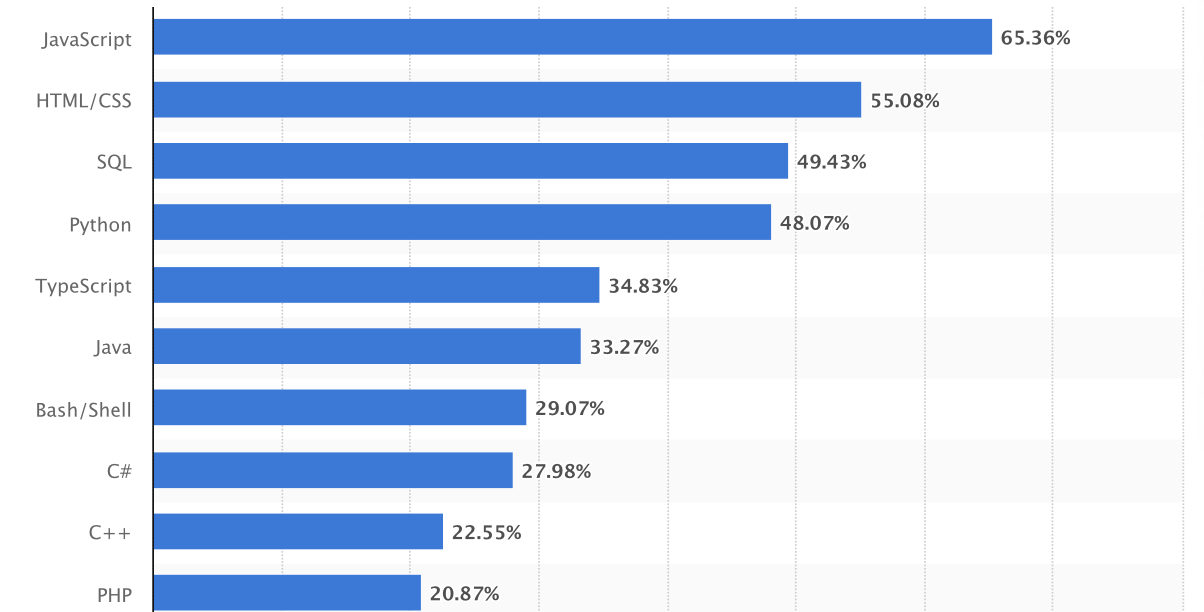
\includegraphics[scale=.65]{atu-computing-latex-template/images/top10Languages.png}
  \caption{List of top 10 programming languages in 2022}
  \label{fig:top10languages}
\end{figure}
It was very important to look at the components that each framework offered within their respective libraries. We understood that we had some requirements to make this application work. When looking at how we would connect the two users, quick response\cite{soon2008qr} codes stood out to us, as they were unique to each individual user. We noted that other applications use them such as Snapchat. How it works on that platform is when a user creates an account they are given a unique QR code which can be accessed from their account page and can be scanned by another user to send a friend request without having to enter a username or phone number. We tested that option and noticed how seamless it was. It seemed to fit our requirement, helped to protect peoples information (an example is not handing out a phone number). Prior to starting this project, we didn't know that QR codes were just a visual representation of text such as a website or a username. \cite{soon2008qr}

We came to the conclusion that React-Native, coupled with JavaScript would be the best option for us as it would be worth learning this language and framework. The statistics tell us that there is a reason JavaScript is so widely used in industry. As we already mentioned already we had some previous experience with JavaScript and to a lesser extent TypeScript, but having to learn an entirely new language to us could cause problems that we would have liked to avoid. In addition, when doing our research to make our decision we noted that the number of resources for React-Native JavaScript development seemed to be greater as opposed to Ionic/TypeScript development. It's is also worth noting that some packages that would be vital to developing this project were easily find-able with a Google search whereas Ionic, not so much. So in the end React-Native with JavaScript was our clear choice. 
\section{Packages}
At the start, we thought that we would need to source a third-party software or a website to do this. The question then was, how do we implement them into our project. Then we came across two packages built into React-Native that could be installed. The first we learned about was react-native-qrcode-svg. This package had the ability to generate a QR code with information that was input by the user\cite{npmQrSvg}. This package did require another dependency though, that being react-native-svg. The purpose of this package was to add svg support to the project\cite{npmSvg}. To add install these packages, you need to run the command either 'npm i react-native-svg' and then 'npm i react-native-qrcode-generator'. NPM was the choice of package manager that we chose to use but more on package managers later. Our reason for choosing a QR code system is that we noticed that restaurants have generally have QR codes inside to bring the user to a web page to view the menu. 

SVG, which is short for Scalable Vector Graphic\cite{cagle2008svg}, is unique type of image format. SVG's doesn't rely on unique pixels to draw it's images but rather uses Vector data which is just an element with a specific magnitude and direction\cite{cagle2008svg}. This type of format makes it a perfect choice for drawing QR codes within our application. You can also have Portable Network Graphic's (PNG's) for a QR code but isn't suitable for the our purposes because if you need to resize a PNG QR code, the image becomes distorted which can result in potential data loss from a generated QR code. We learned that PNG codes are more widely used in industry but we were not able to find any packages on React-Natives website that would allow us to generate PNG QR codes so despite the pros and cons of both, we had no choice but to use SVG generated QR codes. 

The QR code generation library allows the user enter some values to change some aspects to the code that is generated. Most importantly we are able to adjust the size of the QR code on the screen, the color and the background colour which allows for personalizing. We noticed that we would also need a way for the user to be able to save their generated QR code. There is two ways we wanted to go about this. The first was to just save it to the users camera roll via a save button. We learned that there is another package that we could use named 'react-native-fs'\cite{rnfs} with fs meaning File System. To import this package we would run the command 'npm i react-native-fs'. With this command we realised that the user would have a way of saving a QR code without having to take screenshots and then the user having to adjust the size of the screenshot. With this though, the user has to give permission for our application to write the image to their camera roll. 

The other way we wanted to allow the user to have the QR code was to have a button that would send an email with the QR code to the email address that was used to when the user signs up. React-Native has a package to solve this issue we faced named 'react-native-email\cite{npmEmail}'. To install this package we would have to run the command 'npm i react-native-email'. With this package, we would be able to have a email address where the QR code would be sent to, and would also allow us to edit the carbon copy, blind carbon copy, subject and finally the contents of the email itself. With this the user has a way of saving the QR code that they generated locally on their device and also a copy saved to their email address. 

For this application to work, we would need a way for the user to scan a QR code. We again looked at the Snapchat example, which heavily uses the camera on a device as one of its main features. It made sense that we would be doing the same because a QR code is pointless if it cannot be scanned. Once again, React-Native had a library for this, aptly named 'react-native-qrcode-scanner'. Similar to the other packages mentioned, to install this package we had to run the 'expo i Barcode-Scanner' command\cite{barCodeScaner}.

The documentation for the packages Barcode-Scanner and react-native-fs mentions that on iOS devices running iOS 10 or earlier needs to have some code added to info.plist, a file in the iOS folder of the project. We learned that iOS 10 is no longer supported on the App Store (the app for downloading apps on iPhone) so even if this application would put on the App Store, devices running iOS 10 cant even download apps. Since October 2022, only devices running iOS 12 and on-wards can download apps. The latest version of iOS is 16 so there is no chance of this becoming an issue. The reason for this is we needed a way to give permission to user to be able to allow the app to use the camera. 

For this project, we need a way to navigate around the app, say for example when we press a button or an event happens. The React-Native library has a package for this as well named 'react-native-navigation'. This provides 100 percent native platform navigation on both iOS and Android\cite{npmNavigation}. Like the other packages thus far, its installed with 'npm i react-native-navigation'. There really isn't too much to say about this package. You just have to add a Navigation tag into the app.js and import an index.js file that with the different screens which allows the user to move to different screens in a stack format. Each page is rendered on top of another allowing us to go back forth with ease. 

\section{Devices we are developing for}
When developing a mobile application, we need a way to be able to see how the front end looks when we make a change to it. We needed to learn how we would go about that. First we found out what mobile devices we would have access to. We had an iPhone 14 Pro Max and would be developing the application on MacOS Monterey 12.6. We looked into obtaining an Android device but that was not possible. We learned that both Apple and Google offered simulators that would run on our machine but for both platforms, this required some setup to get this to work. Prior to realizing, getting an Android device was not possible, we did find out how we would go about that.

For Android, we would have needed to install Android studio\cite{meetAndroidStudio} the official Integrated Development Environment (IDE) for Android app development. Even though this is a code editor, we wouldn't actually use this to write our code (we used Visual Studio Code but we will discuss that later) and just needed to get the Android Emulator. From the documentation we learned that you would install the emulator through Android Studio by choosing the Android version we would like to develop for\cite{installAndroidStudio}. We also needed NodeJS, an open source server environment for running the application. After setting up Android Studio, we would have needed to create a React-Native application within a folder in the terminal with the command 'create-react-native-app Tipper', select which platform we would be developing for. Finally when that was all done, run the command 'npm run android'. Below is an example of what this may look like. Also Yarn is a package manager like NPM. We used NPM for this project.
\begin{figure}[h]
  \centering
  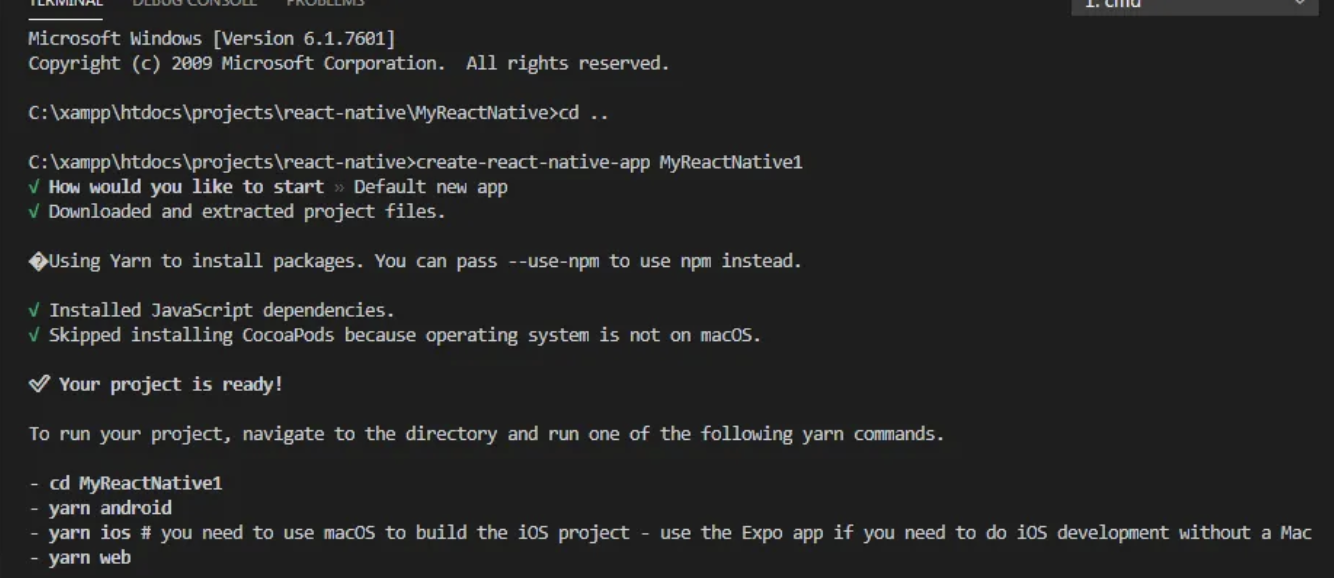
\includegraphics[scale=.55]{atu-computing-latex-template/images/Screenshot 2023-04-18 at 19.08.30.png}
  \caption{Setting up a react-native project}
  \label{fig:{Setting up a react-native project}}
\end{figure}
And by running the command 'npm run android', we would see something similar to this. 
\begin{figure}[h]
  \centering
  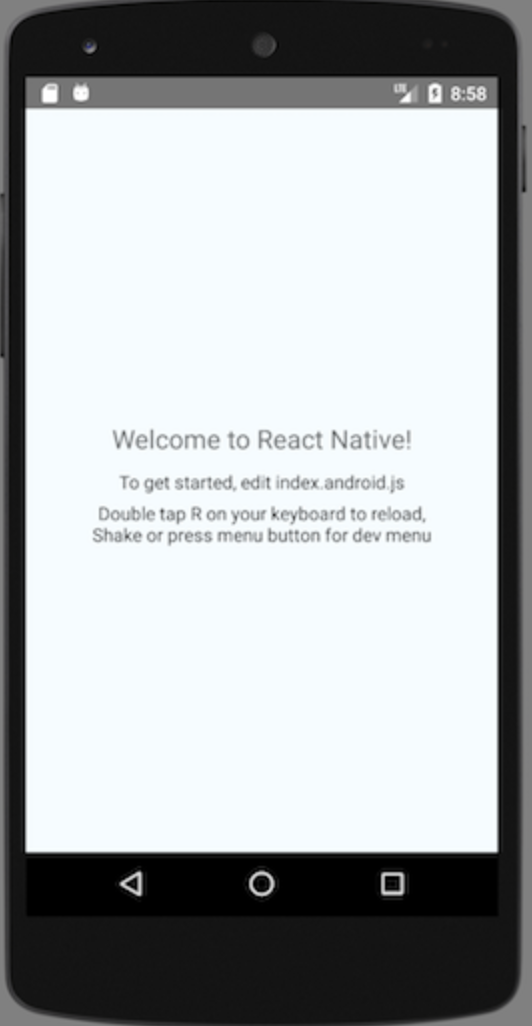
\includegraphics[scale=.55]{atu-computing-latex-template/images/Screenshot 2023-04-18 at 19.13.37.png}
  \caption{Android Emulator running}
  \label{fig:{Android Emulator running}}
\end{figure}
\section{Setting up the development environment}
The process setting up an iOS simulator is quite similar but we learned that there were some caveats for this. Firstly, like developing for Android which requires Android Studio, you need to download XCode, Apple's integrated development environment for MacOS and MacOS only unlike Android Studio, can be installed on Windows, MacOS, Linux and Chrome OS. Written in C, XCode is touted as being much faster with a twenty-five percent increase in project build speed with the latest version (that being XCode 14)\cite{XCode} and with "simplicity and power of Swift and SwiftUI with a new multiplatform app experience". Then when looking at forums and discussions about XCode where we observed multiple threads about XCode's poor performance, crashes and unusual errors. 

We have to admit this did become a cause for concern. We were building this application on a base model, 2019 MacBook Pro with 1.4 GHz Quad-Core Intel Core i5 CPU and 8GB of 2133 MHz LPDDR3 Random Access Memory and 256 Gigabyte Solid-State Drive. We also noticed that users who had an improved performance experience of XCode were running Mac's with Apple's in-house built Sillicon chips where as our machines were running Intel chips. The size of XCode to install was around 11.7 Gigabytes but required the install device to have around 40 Gigabytes free on disk. That wasn't even the end of it. The more versions of iOS and Simulators we installed, the install size grew fast. The reason for the massive size is the fact that XCode supports MacOS(Desktop/Laptop), iOS(iPhone), iPadOS(iPad tablets) and TvOS(Apple TV's). Then on top of that, each device having multiple versions of their operating systems having different simulator runtimes, libraries, compilers, and software development kits.

When it came to setting up the simulator for the iOS devices on our machine, we had to jump through a few more hoops. First of all we needed a package manager. We had three options for doing this. The first was Node Package Manager or NPM. The second was Yet Another Resource Negotiator or Yarn and finally Homebrew. They all essentially did the same thing. Homebrew was only available on MacOS. NPM was the package manager that we had previous experience with and Yarn we never used before. The main difference between NPM and Yarn is NPM installs packages sequentially where Yarn installs dependencies in parallel. A smaller difference was when installing a package, was simply if you said either npm install or yarn add. Although to install NPM or Yarn on MacOS, we would have needed to use Homebrew. 

The next step we needed to do was install Node.js\cite{setUpDevEnviro}. Upon doing this we we realised that Node.js was already installed on our machine from working on previous projects. How we knew this was running the command 'node -v' in the Terminal. If it was a case that we didn't have it installed, we would have needed to download from the install file from the Node.js website.

Next we installed Watchman, a piece of software that detected changes to code and refreshed the simulator to show this\cite{setUpDevEnviro}. Say if we changed the colour of a button in our application, the simulator automatically refreshed and was displayed to us. Next we needed XCode installed on our machine which we got from the App Store. Upon installation, we installed a simulator by selecting the iOS version we wanted in the components settings. Next was install Ruby (which was also already on our machine) and Cocoapods. The reason for this, when we would install a package, we needed to link the package to the iOS device, also known as Pods\cite{setUpDevEnviro}.

Finally, we created the React-Native project using it's Command Line Interface(CLI)\cite{setUpDevEnviro} with the command 'npm react-native@latest init Tipper'. This generated our project and all of the files that we would need to start development. Then to run the iOS simulator we ran the command (from the projects root directory) 'react-native run-ios'. This will open the XCode simulator\cite{iOSSimulator} and start to build the project. Initially we found the build process painfully slow. We later discovered that the reason for this was the folder was stored on iCloud Drive, Apple's cloud storage solution and was trying to sync everything over the internet which killed our performance. What we saw was nearly identical to running the Android Emulator but showed an iPhone instead of an Android device.

For the Integrated Development Environment (IDE), we chose to use Visual Studio Code which is a rich-text editor. A lightweight code editor that runs on MacOS, Linux and Windows\cite{VSCode}. When it came to choosing an IDE, we wanted to use something that is reliable and easy to use. We were very familiar with Visual Studio Code from working on previous projects over the course of our education. That isn't to say that we didn't at least explore other options. As mentioned before XCode was an option that we could have used but because of the reasons mentioned before, we chose not to go with that.

Visual Studio Code also offers customisable features in the form of plugins for developers to curate a pretty selective development environment. Along with built-in support for Node.js, TypeScript, and JavaScript, it quickly stood out to us as a choice for developing our project with.

Next we decided to look at Android Studio. We looked at what it had to offer but quickly decided against this. Mainly because that Android Studio is used primarily for development on Android devices\cite{meetAndroidStudio} which we would not have access to any devices to properly test outside of the simulator. This was important because the package 'react-native-qrcode-scanner'\cite{npmQrSvg}, which scans the QR code using the camera, will only work on physical devices and not on Android's emulator or XCode's simulator. We would need access to a camera and neither can provide this. 

Finally we looked at Visual Studio, the 'big brother' to visual studio code (both are Microsoft products). This is an actual Integrated Development Environment which offers features such as editing, debugging capabilities, code completion tools, compilers and graphic designers\cite{VS}. Visual Studio can come in a free and paid version as opposed to Visual Studio Code which is free regardless. Both also have their own benefits and drawbacks. Visual Studio's performance is noticeably slower (we have first hand experience of this) where as Visual Studio Code's IntelliSense (Code auto-completion) is worse. The one thing that stood out to us was the install size difference between the two. Visual Studio Code uses around 500 Megabyte\cite{VSCode} where as Visual Studio can take anywhere between 2.3 Gigabyte and 60 Gigabytes\cite{VS}.

When we took everything into account between performance speeds, install sizes and the features that is offered, Visual Studio Code was the clear choice to develop our project with. We can speak from first hand experience that Visual Studio is slower in comparison to Visual Studio Code, XCode's performance was also not favourable on our machine and Android Studio did not meet the requirements the decision we felt was not difficult to make. 
\section{Choosing a database}
The next technology that we needed to make a decision on was the database we would use to store our information. We knew that this would primarily be used for storing login information and maybe some smaller pieces of data, e.g. a users QR code. At the start we thought that MongoDB would be a good choice. MongoDB is a document database\cite{mongodb} that could be used at any scale. The data is stored in JSON like objects and used multiple massive tech companies such as Google, eBay and Electronic Arts. Before also making the decision on how we would store payments, we learned that MongoDB recently started supporting multi-document transactions. These are atomic (meaning all-or-nothing)\cite{mongodbTransaction}. So if a transaction commits, the data changes made in the transaction are not visible outside the transaction.

We soon learned of third-party services that would handle the transactions that being Stripe (discussed below) and other databases that would handle the login/security features and resetting of passwords using built in methods. This seemed like a good idea to use. Another reason for this is we learned that MongoDB was more suitable for desktop applications in comparison to mobile applications. The option that stood out to us was AWS Amplify, a database solution that is owned by Amazon and is apart of Amazon Web Services that lets front-end web and mobile developers easily build, ship, and host full-stack applications on AWS. Setting up Amplify seemed quite straight forward. The documentation said that all we would need to do is a few steps. The first was to install AWS Amplify CLI, then setup a database and set the data models used signing up and for authentication\cite{amplify}. 

When you hit deploy at the bottom of the page, you are presented with a command that is unique for your database. Run that command in the root folder of the project. Finally copy the configuration code also presented with the command into a config.js file. From there you have access to methods such as 'signUp()', 'forgotPassword()' and 'signOut()' by adding import Auth from 'aws-amplfy' . Overall it seemed straight forward enough. The documentation was thorough and detailed. AWS also had videos showing us how to get this setup. 

Amplify offers other features such as push notifications, Artificial Intelligence and Machine Learning predictions, different data storage solutions and REST API's. Amplify proved to be a robust choice for our back-end that would allow us to expand the project in multiple ways if so we chose too while also satisfying our needs for what we needed at the moment\cite{amplifyFeatures}.
\section{Transactions}
Finally, we needed to decide on the way we would process payments from one user to another. First we thought about using Apple Pay but soon decided against this. Implementing Apple Pay required us to sign-up for an Apple Developer account, a merchant identifier along with other hoops to jump through\cite{ApplePaySettingUp}. We also didn't want this application to become Apple dependent. We were already developing on MacOS, XCode and for iOS. We felt it would be best to try and incorporate as many unique technologies as possible. That is when we came across Stripe, an Irish-American company that on their website, says works with startups to large enterprises. We seen that they offered solutions for everything we needed and more. We admit that we were skeptical as we never worked with something like this before (money and security) so we had to base everything we knew off of online discussions and what was on Stripes website\cite{stripe}. From what we learned implementing Stripe would be far easier and meant that we were not tied to Apple Pay. This also meant that we could expand to other platforms easier. We knew that we would need to use ExpressJS(back end web application framework for building RESTful API's) and Node (Node.js is a back-end JavaScript runtime environment) because to connect to Stripe, we need a simple server that can contact Stripes servers to start a transaction when they payment flow is called. Stripe is implemented using a 'Secret Key' to connect to our Stripe dashboard and a public key that is called when a transaction is going to be made.
\chapter{System Design}
\section{Login and Authentication flow}
From our research, like looking at Snapchat which has some similarities to our project (login and camera functionalities) we understood that we had a good template to reference as to how our project should be structured. Snapchat (and most mobile applications) have the same screen stack. The first page a user who has not signed in before should see a screen that allows them to either sign in, create an account or reset their password. We decided that the user needs an entry box for both the username and password and then buttons for the other functionality on the screen. From here the user has options to do everything they need. We also wanted to include that app title on the page. 
\begin{center}
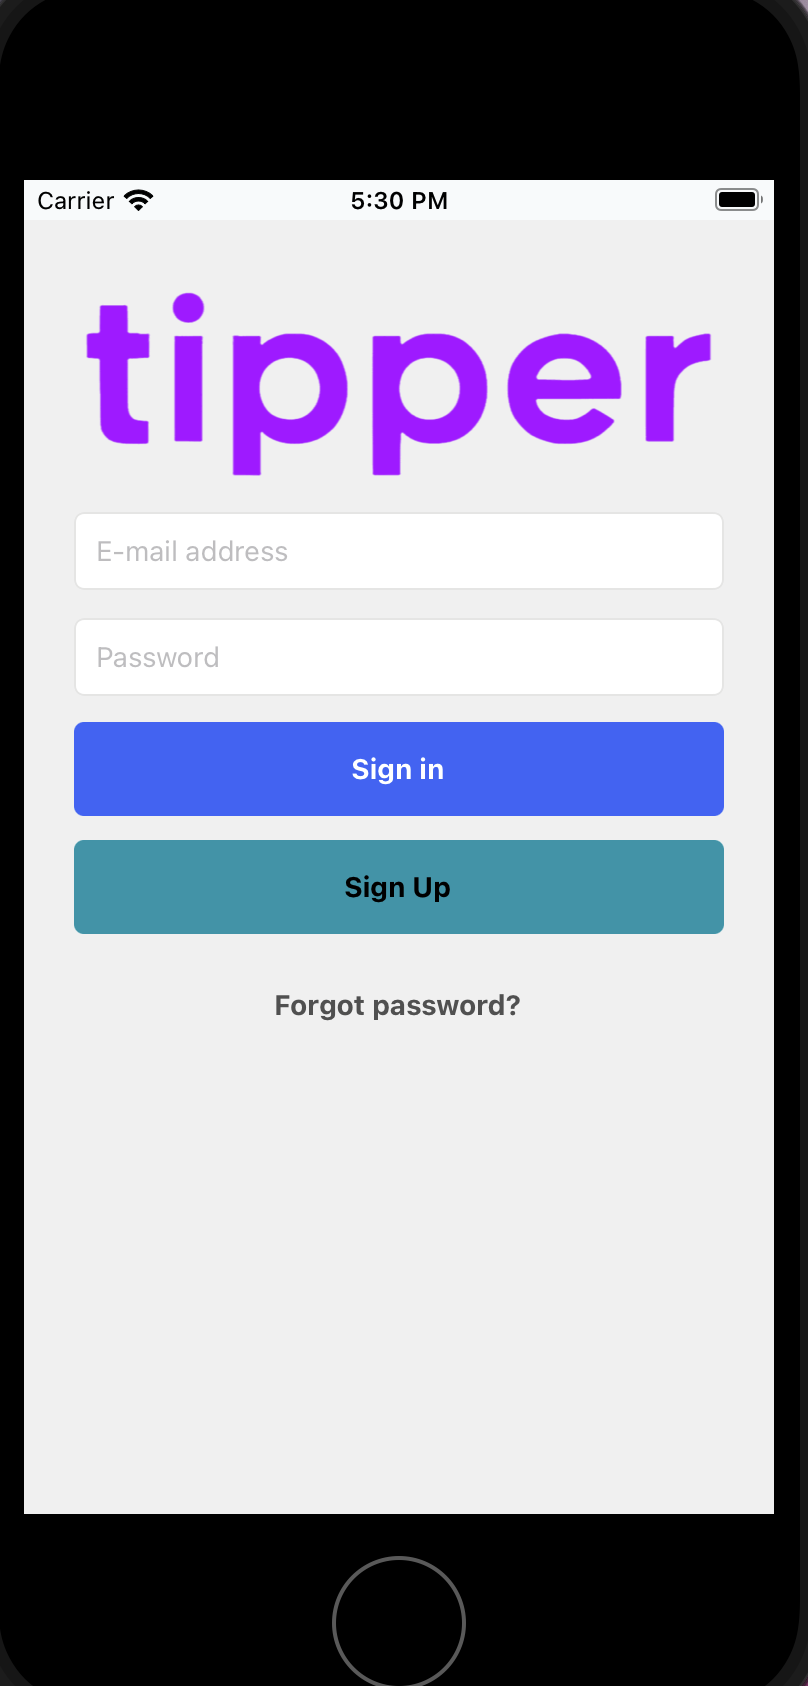
\includegraphics[scale = .40]{atu-computing-latex-template/images/SignInScreen.png}
\end{center}
When the user wants to create an account, they must tap the 'Sign Up' button. From there they are presented with two buttons. Either to sign up as a customer or an employee of a business. If the user decides to sign up as a customer, they are presented with input boxes for First Name, Second Name, Email Address, Phone Number and Password. The phone number isn't used for any authentication but keeps in line with the ability future additions to the app. The password has to include an uppercase, lowercase, a number and be at least eight characters in length.
\begin{center}
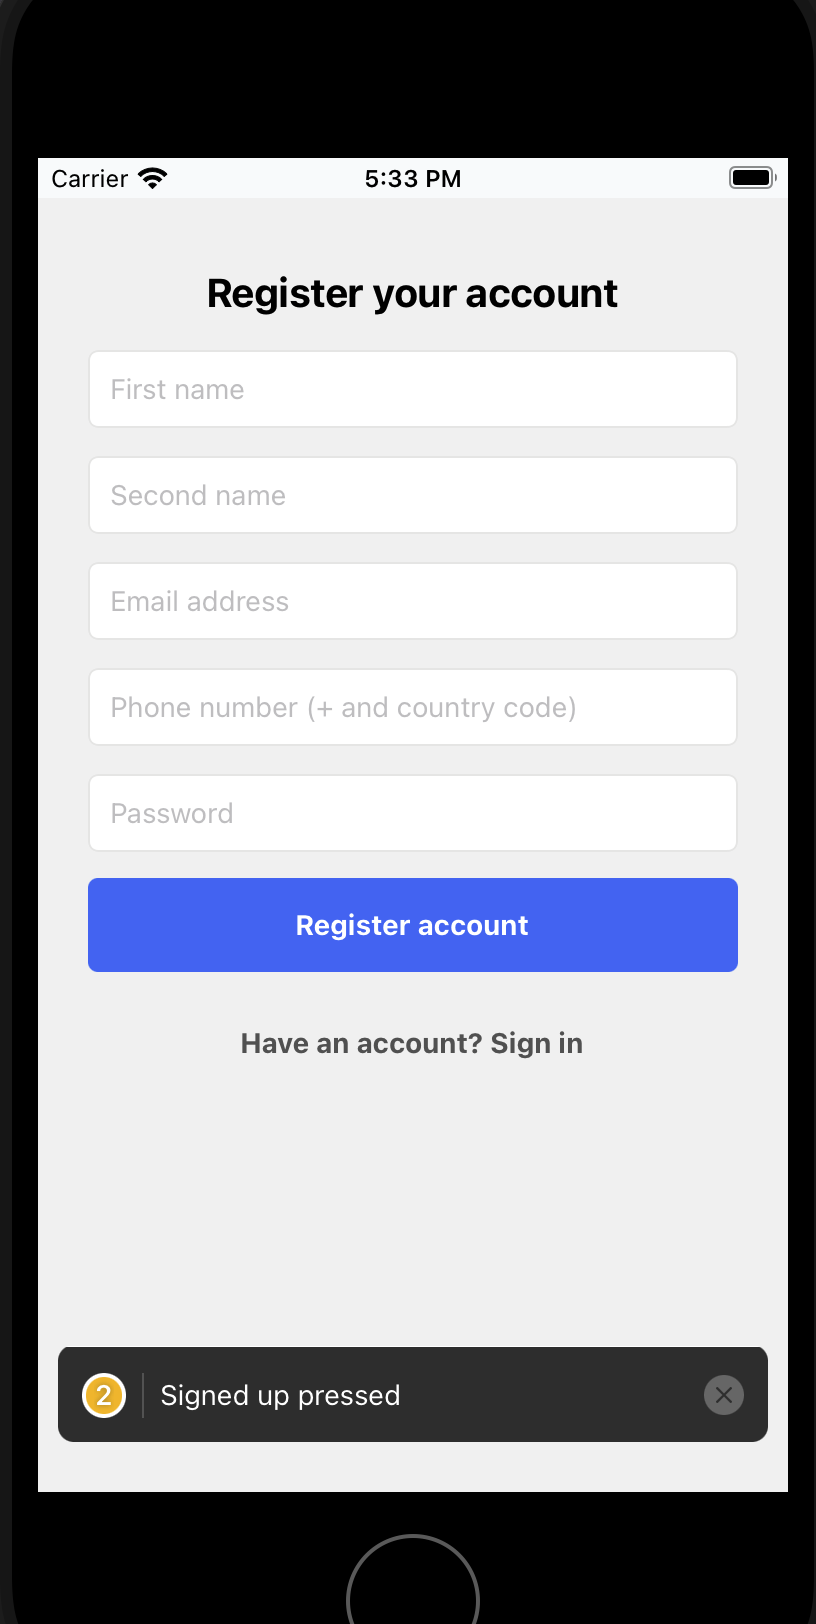
\includegraphics[scale = .40]{atu-computing-latex-template/images/SignUpCustomer.png}
\end{center}
Then the user must press register account button to be brought to a page where they must enter a verification code that is sent to them via email (one of the methods provided by AWS Amplify) and can get the code resent them via email again which is another methods provided. If pressed, this makes the previous verification code invalid. Once the valid code is entered, the user is then automatically brought back to the sign in screen. 
\begin{center}
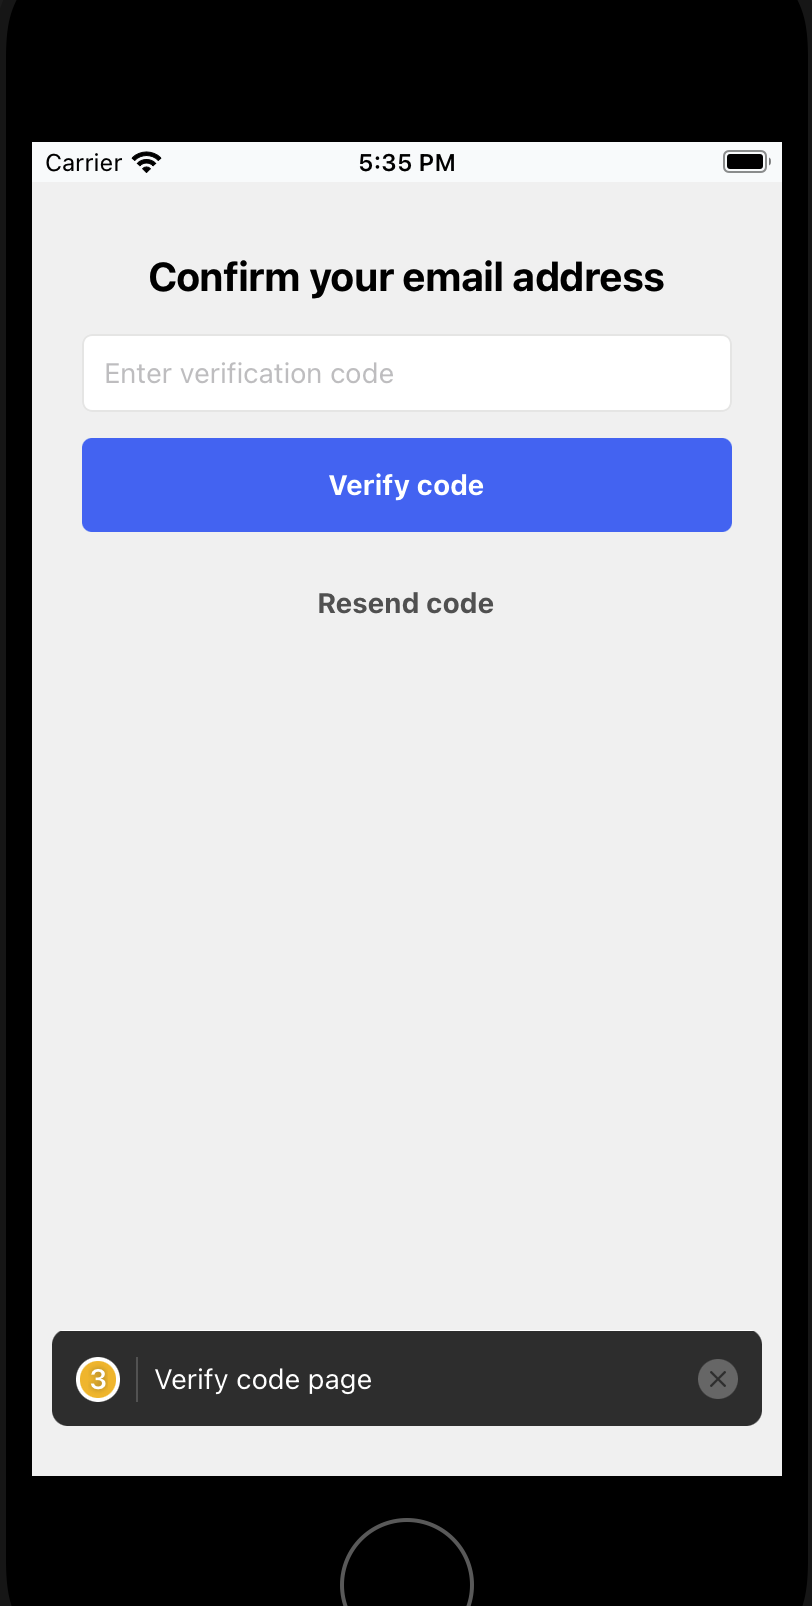
\includegraphics[scale = .40]{atu-computing-latex-template/images/ConfirmEmailCode.png}
\end{center}
On the other hand, if the user wants to sign up as an employee, the sign up process is slightly different. The entry boxes are the same as the customer sign up flow with the same button functionality. 
\begin{center}
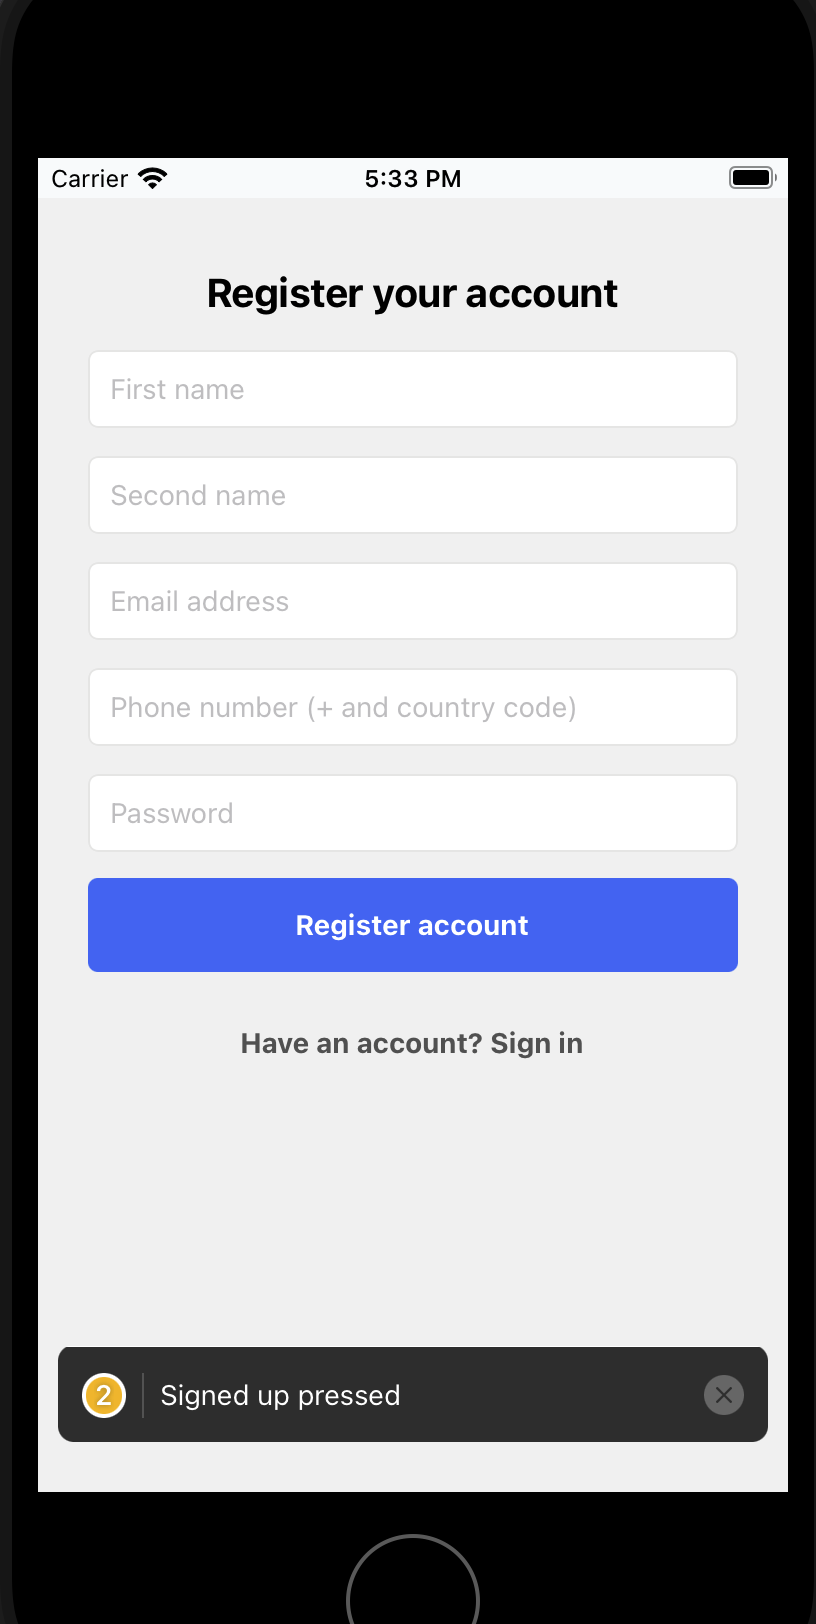
\includegraphics[scale = .30]{atu-computing-latex-template/images/SignUpCustomer.png}
\end{center}
They are then asked to enter the verification code and when the user has entered a valid verification code,
\begin{center}
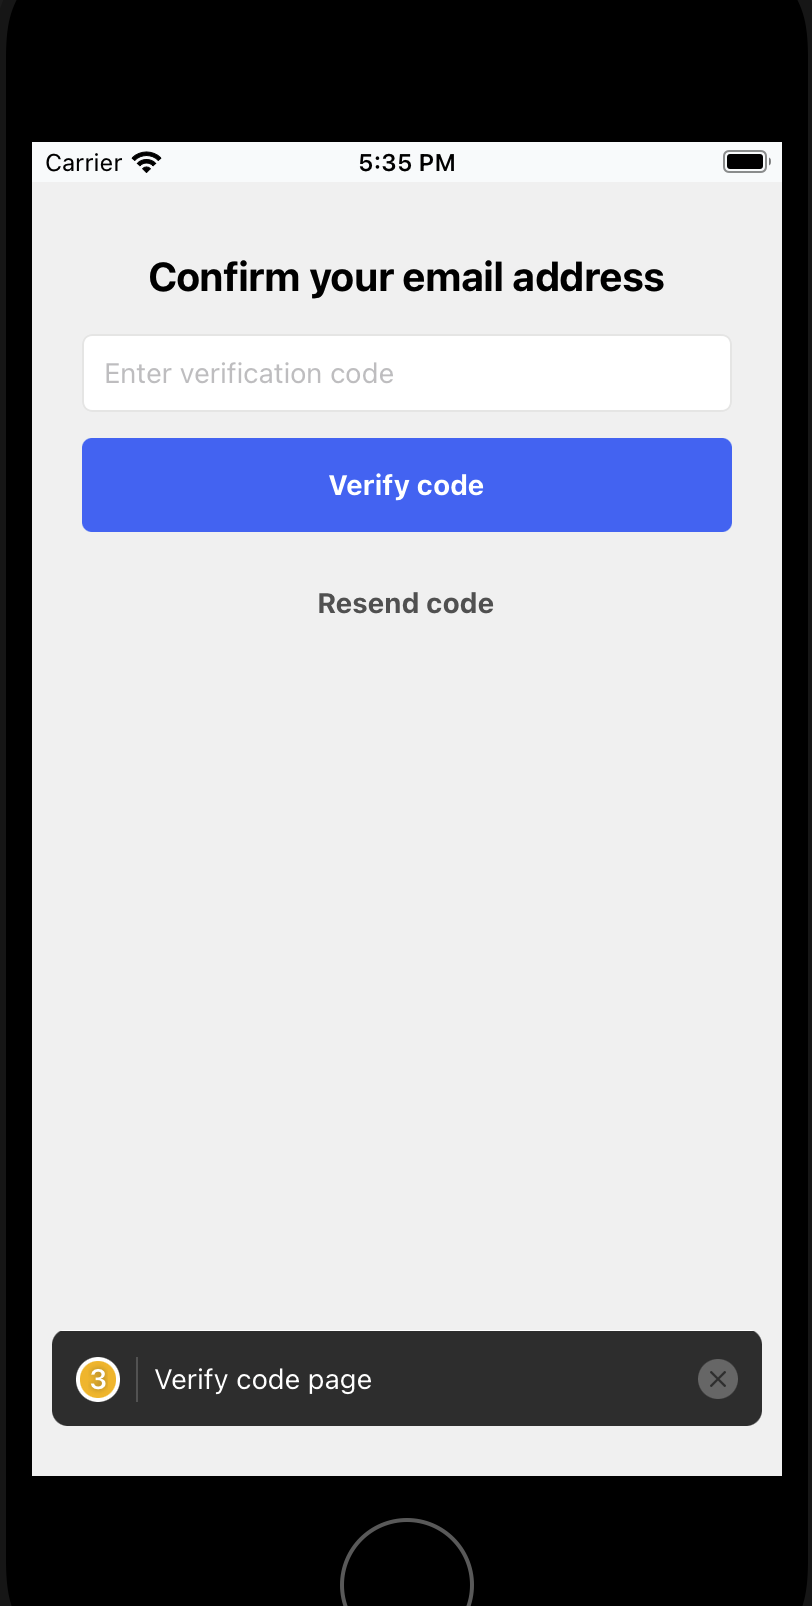
\includegraphics[scale = .40]{atu-computing-latex-template/images/ConfirmEmailCode.png}
\end{center}
The user is then brought to the QR Code generation screen. From here the user can enter their IBAN and hit a button to generate their unique QR code. They user can keep generating another QR code if they make a mistake. On this page the user also has the option to either save the QR code to their device, although this requires permission from the user to do this. The user can also send their QR code to the email address that they used when creating their account. Both of this happens when the respective button is pressed. After the user is happy, they hit the finish button to return back to the sign in screen. 
\begin{center}
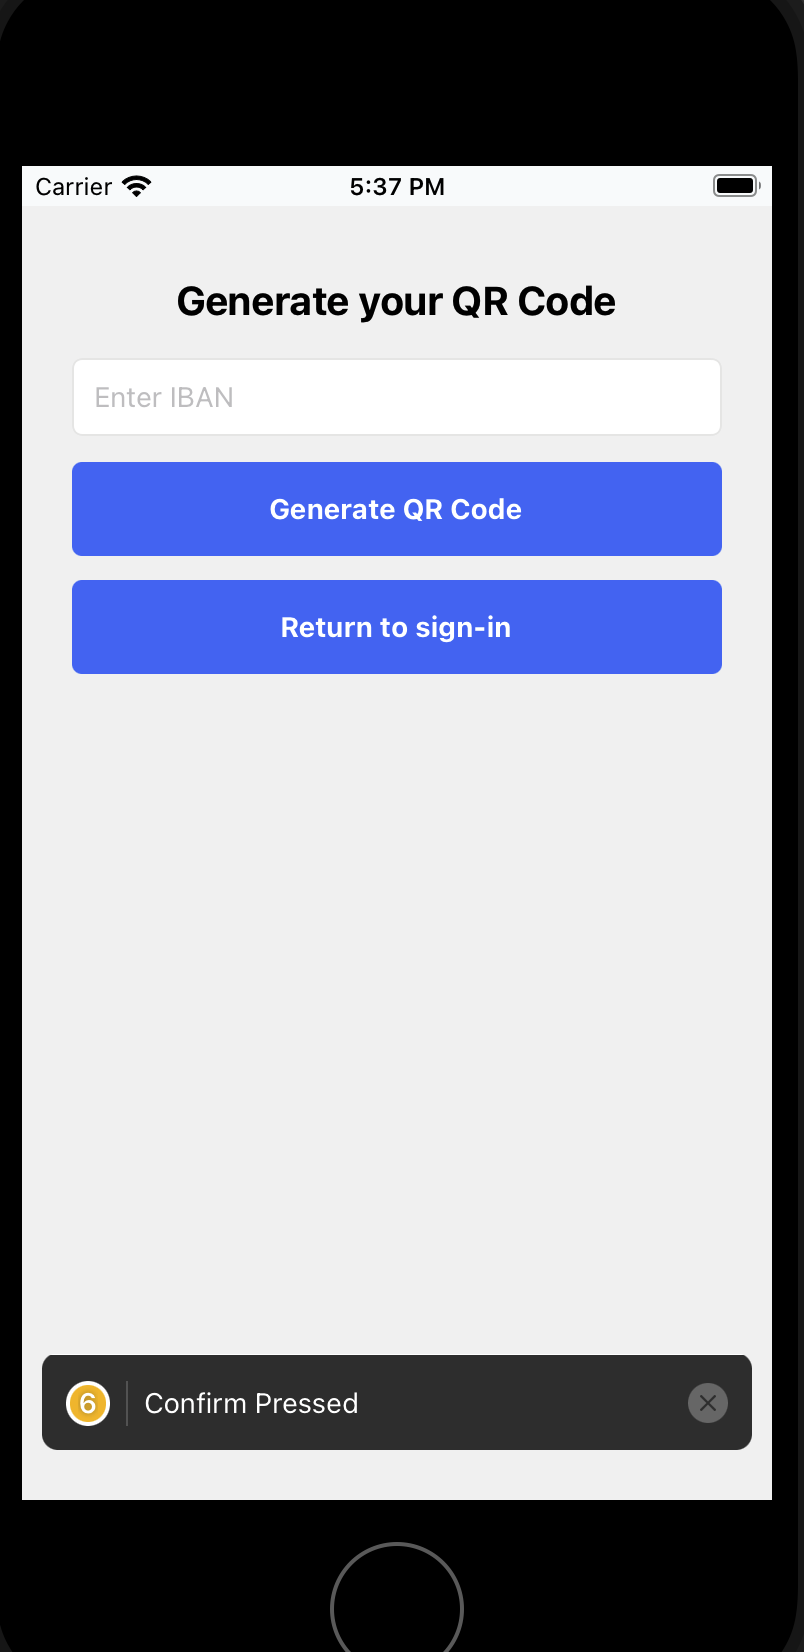
\includegraphics[scale = .40]{atu-computing-latex-template/images/GenerateQRCode.png}
\end{center}
Finally, on the sign in page is the option to reset their password by pressing the forgot password button. From here the user is asked to enter a valid email address of the account they would like to reset their password for. On this page the user presses a button to progress and is sent a verification code. 
\begin{center}
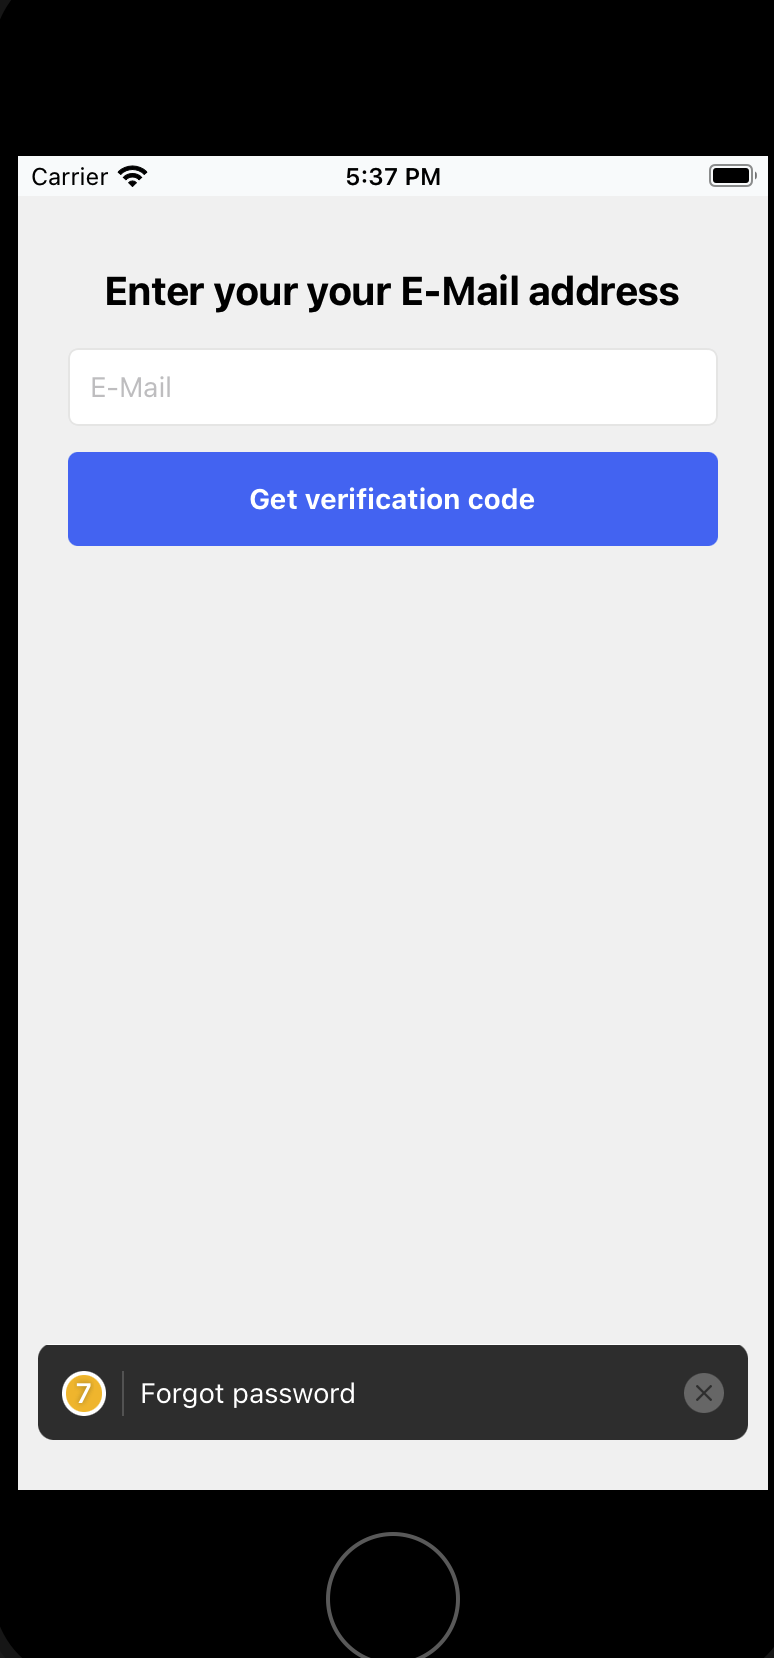
\includegraphics[scale = .40]{atu-computing-latex-template/images/EnterEmailReset.png}
\end{center}
On the next screen the user must enter a valid verification code that has been sent to their email address and the new password. The user can also request a new verification code as well. Once the verification code and password requirements have been met, the user will returned to the sign in page.
\begin{center}
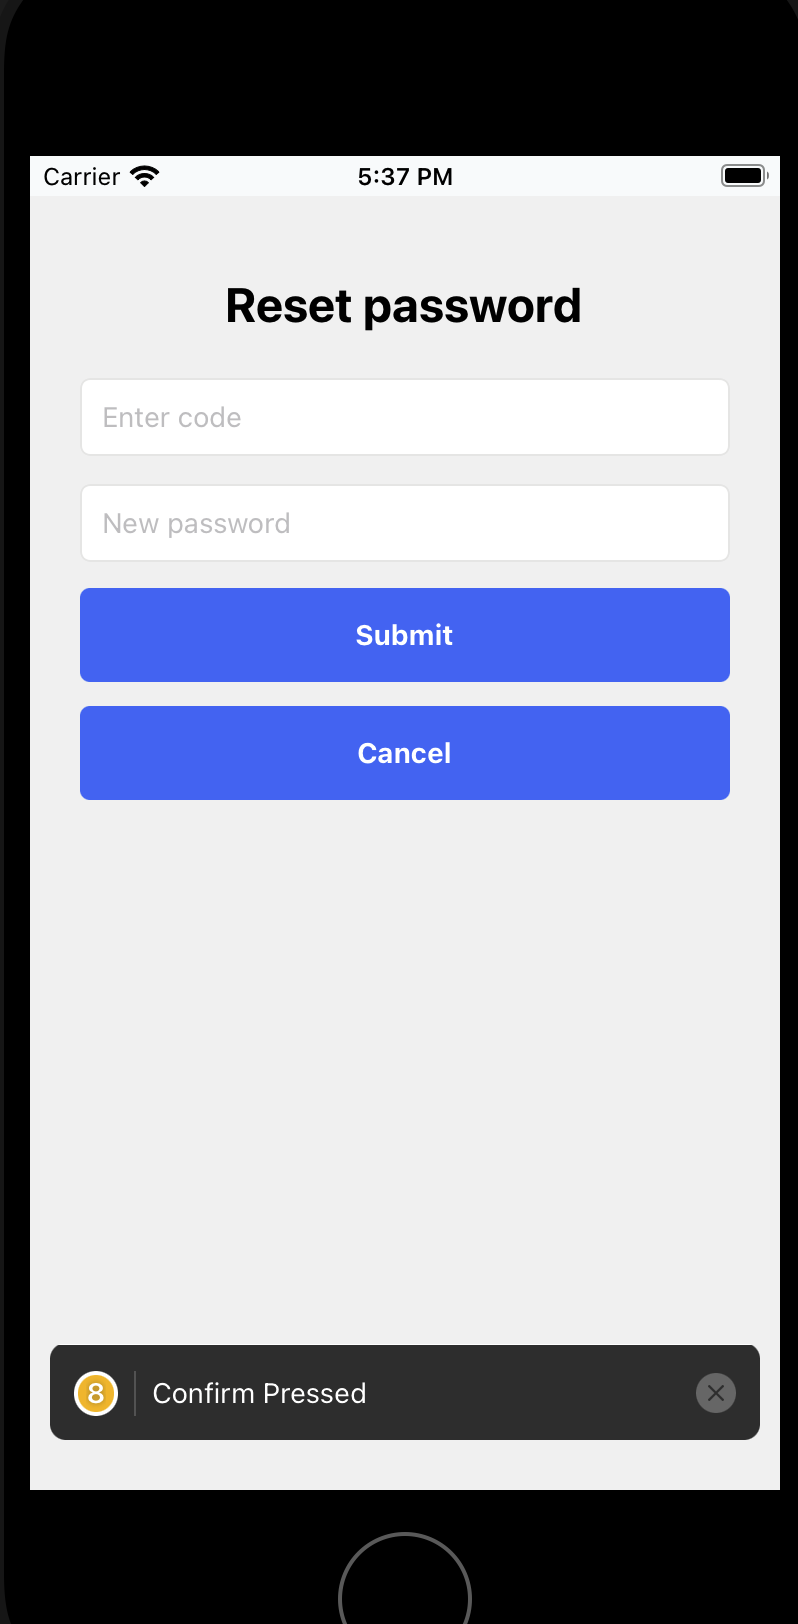
\includegraphics[scale = .40]{atu-computing-latex-template/images/EnterNewPassword.png}
\end{center}
Here is a complete UML diagram showing the entire authentication flow
\begin{center}
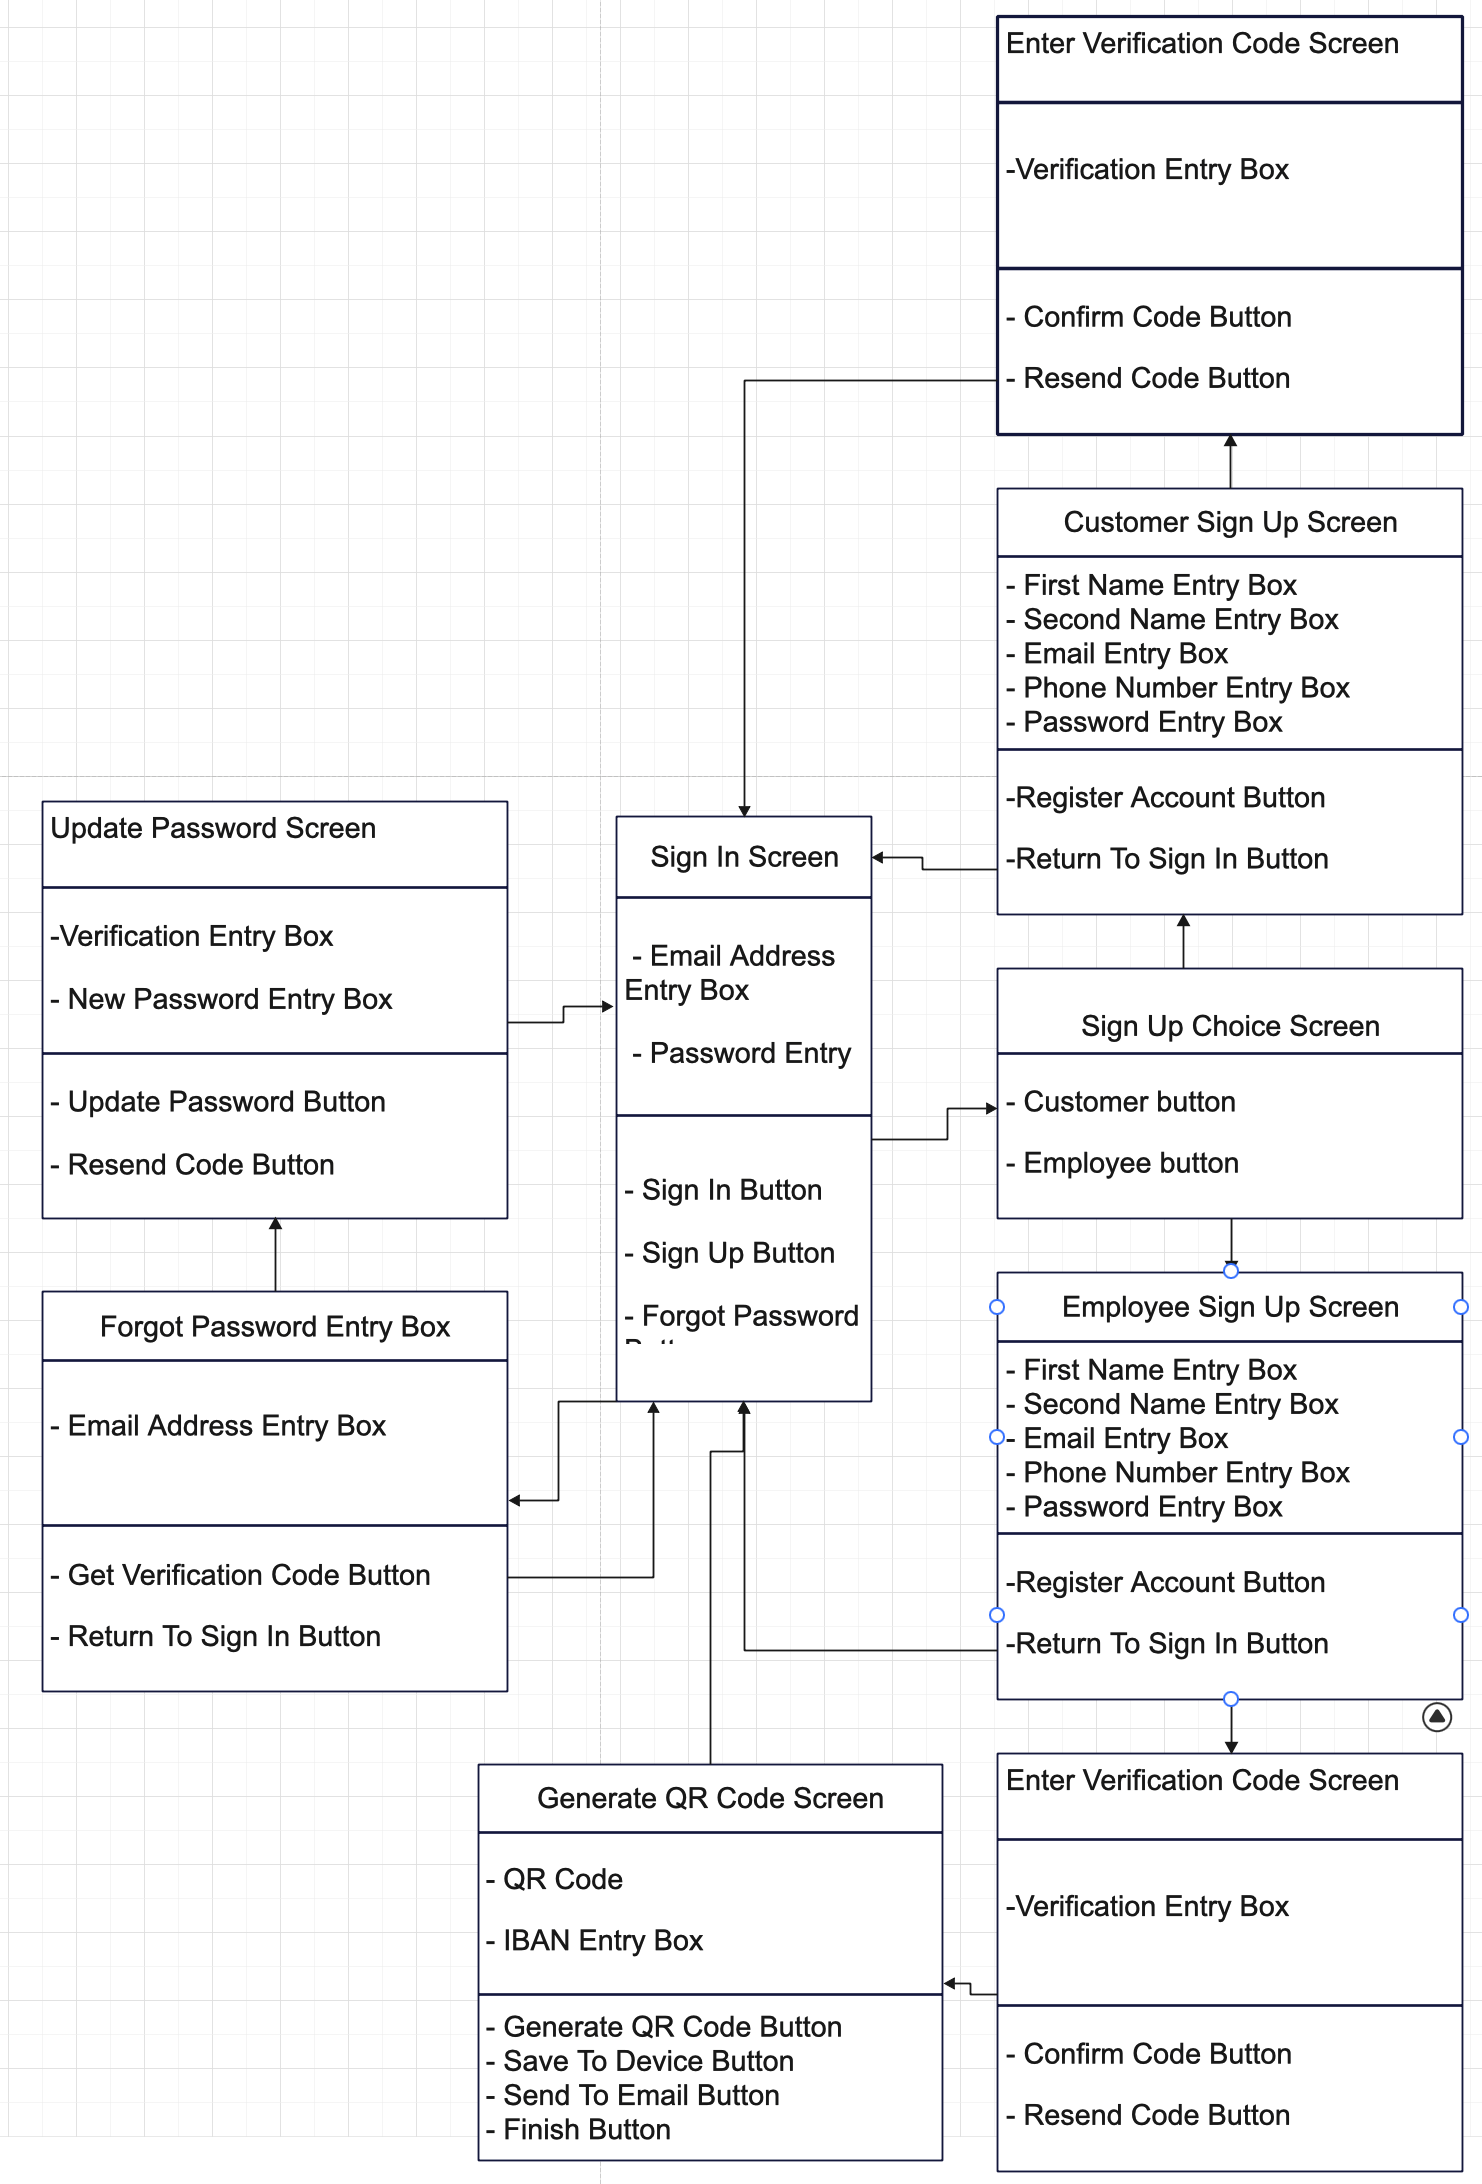
\includegraphics[scale = .40]{atu-computing-latex-template/images/Auth UML.png}
\end{center}

\section{Homepage and updating user details}
When the user logged in they are met with three options. They can either make a tip, updated account details or sign out. To start, if the user wants to update their email address or their password they tap 'Update account details'. If the user does this, they are met with two options, 'Update email' or 'Update password'. Both have a similar flow. The user just needs to enter a new email or password depending on the option they have chosen and tap the button to make the change and is then brought back to the home page again. For the purposes of security, the user must enter their old password along with the new password to update to a new one. The reason for this being added to the application is the user needs a way to update their information after being logged in. It means they don't have to go through the forgot password authentication route.

\begin{center}
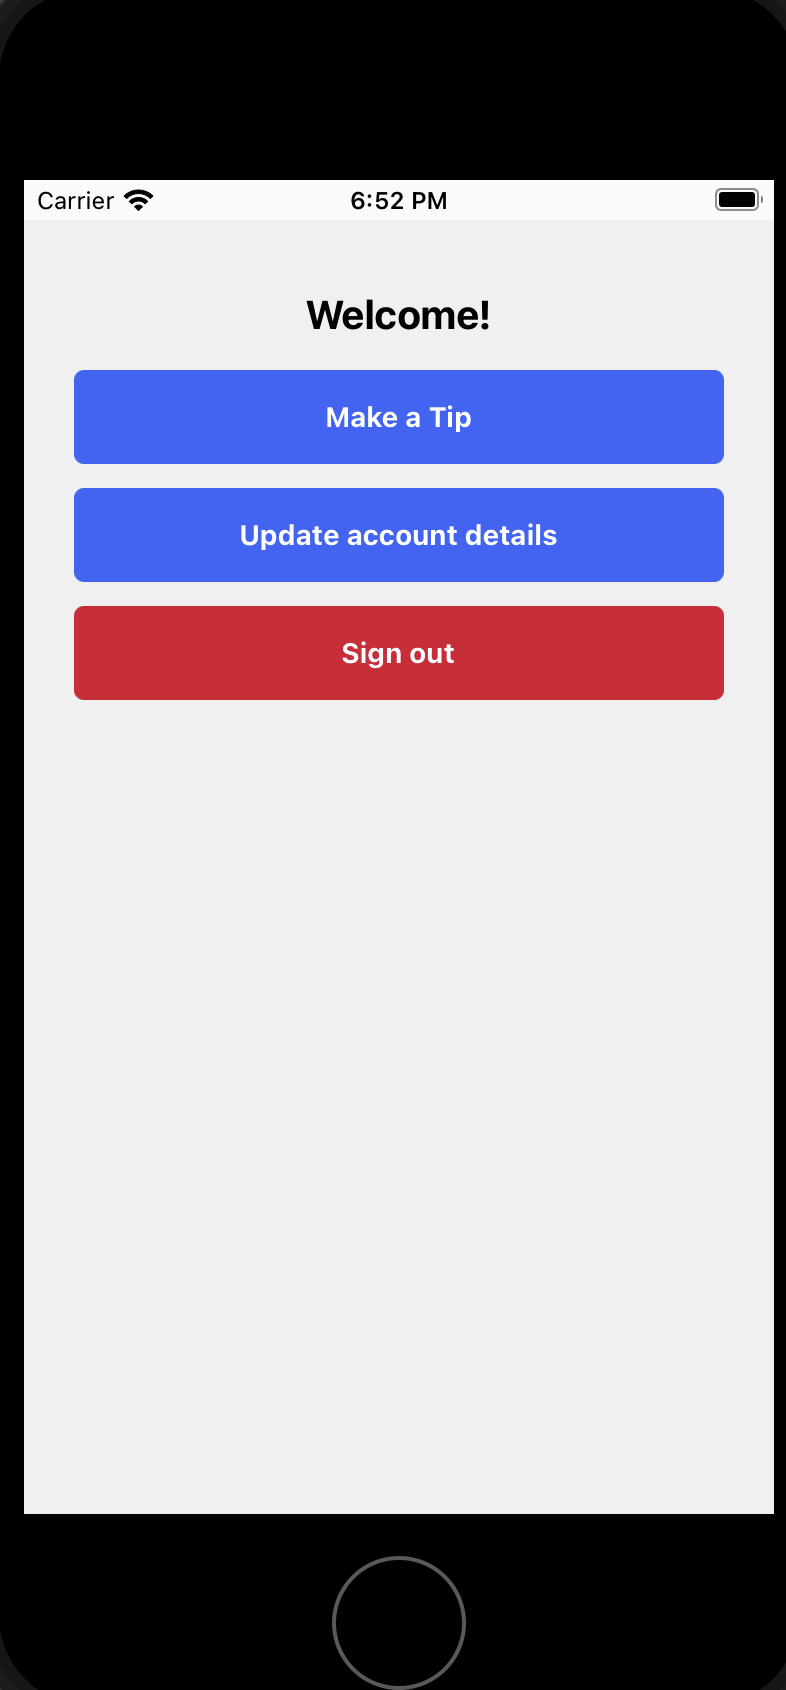
\includegraphics[scale = .40]{atu-computing-latex-template/images/Homepage.png}
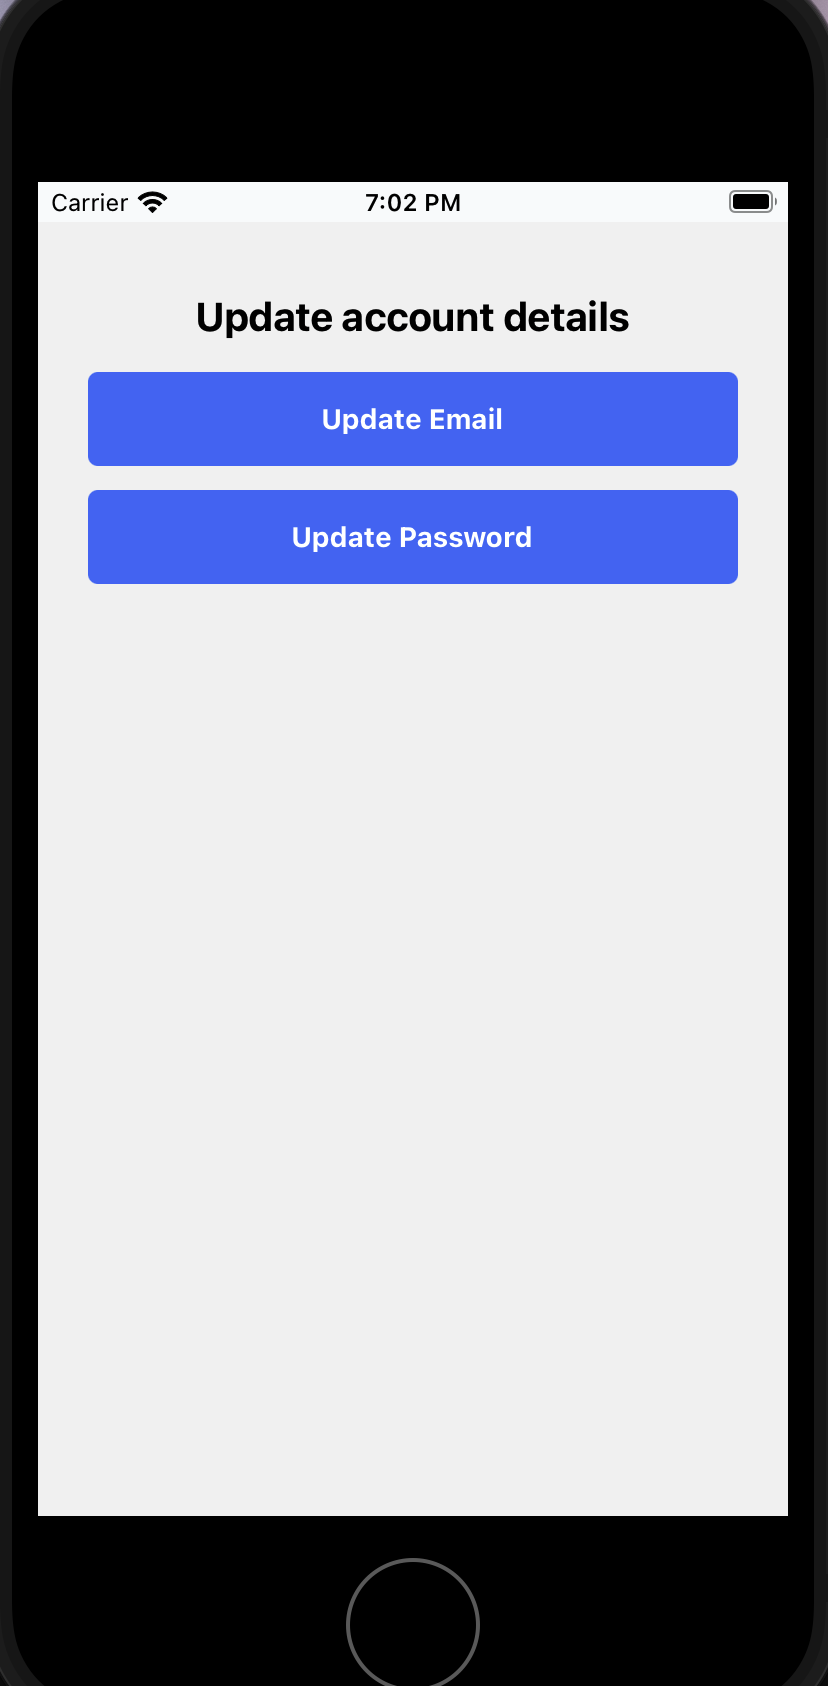
\includegraphics[scale = .40]{atu-computing-latex-template/images/UpdateInfoChoice.png}
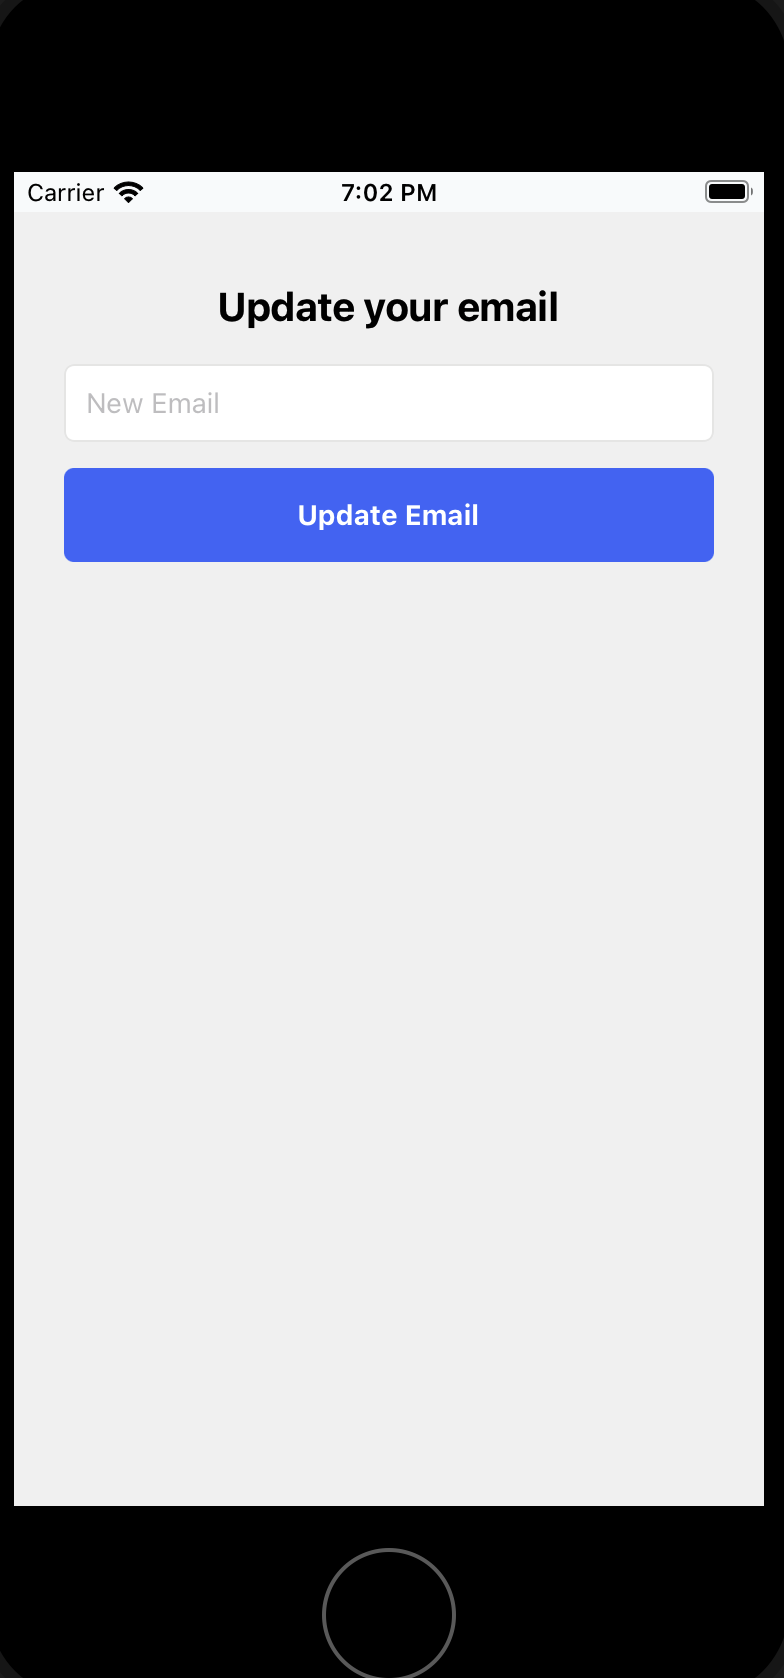
\includegraphics[scale = .40]{atu-computing-latex-template/images/Update email.png}
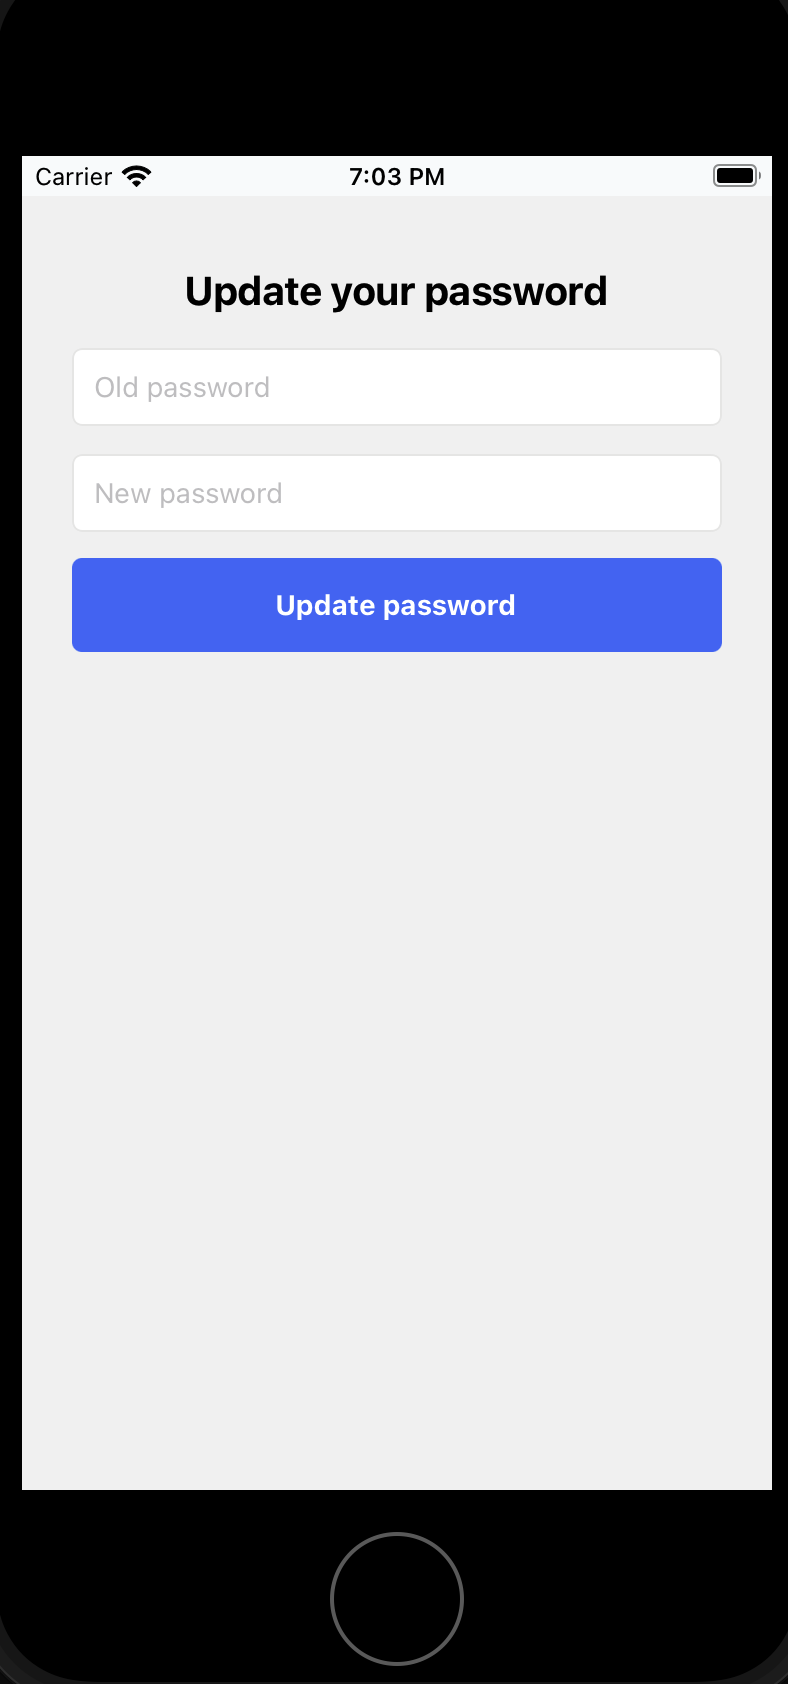
\includegraphics[scale = .40]{atu-computing-latex-template/images/Update password.png}
\end{center}
\section{Tipping  flow}
When the user is on the homepage and decide to make a tip, they tap the Make a Tip button. From there the user is brought to a new screen with two entry boxes, Enter Bill Total and Tip Percentage. After the user has done this, they can tap a button to calculate the tip and they keyboard will disappear. When the user calculates their tip, the calculated tip is presented on screen with a euro symbol beside it. When the user is happy with the amount they would like to tip they tap the Scan QR code button which will open a screen for the user to scan the QR code. If the user has never used the application before, they must give permission to allow camera access. This is what was added to the info.plist file.
\begin{center}
    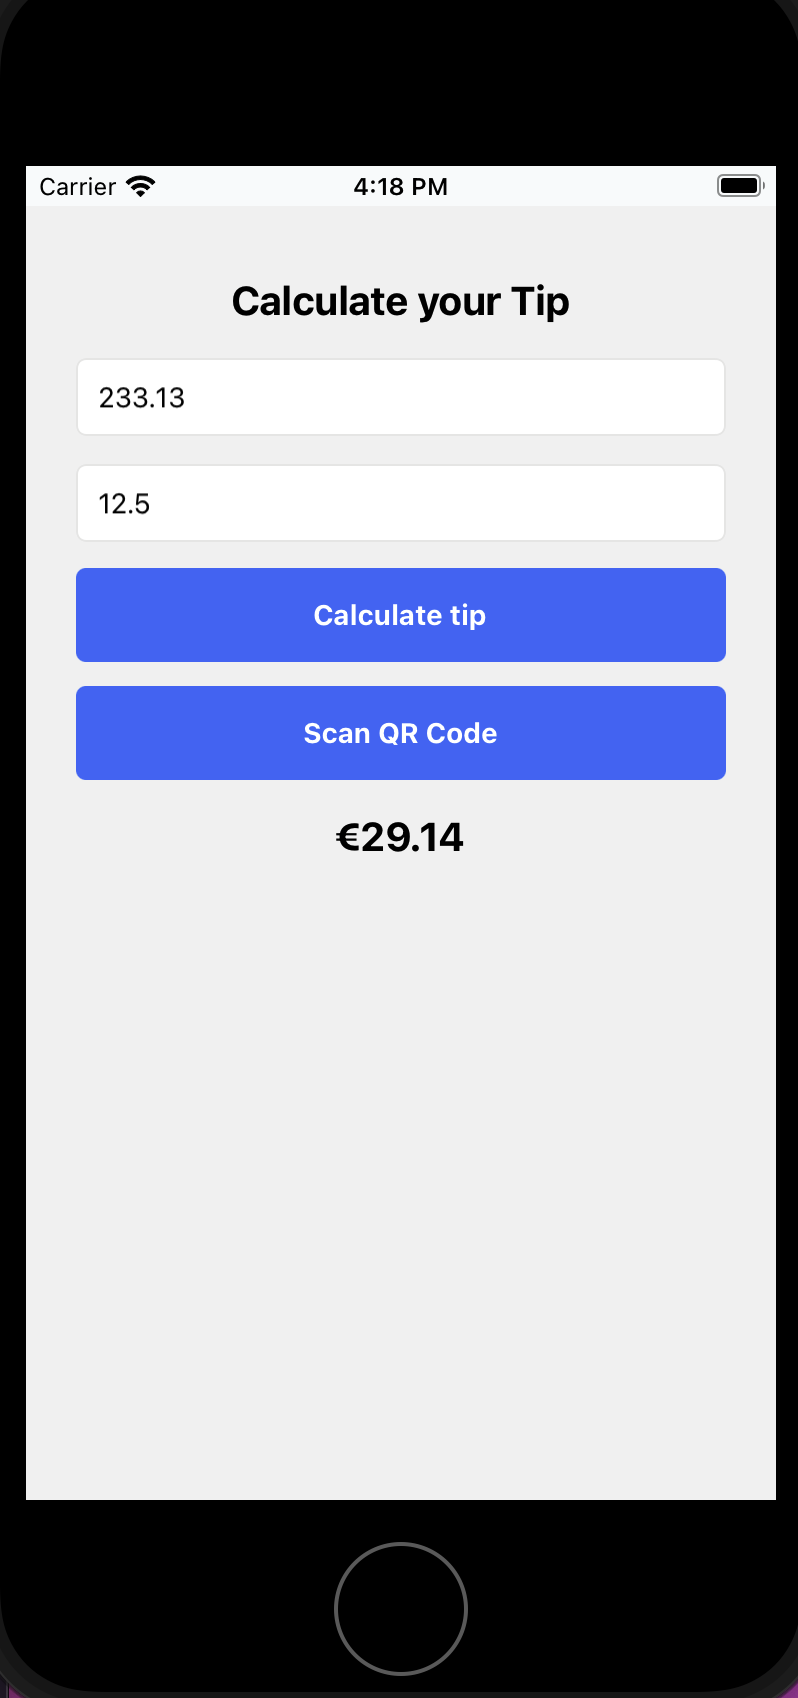
\includegraphics[scale = .40]{atu-computing-latex-template/images/CalculateTip.png}
\end{center}
Once the QR Code has been scanned, the user is brought to the payment screen where they confirm the payment MORE ON THIS
This is the UML diagram for when the user has signed in.
\begin{center}
    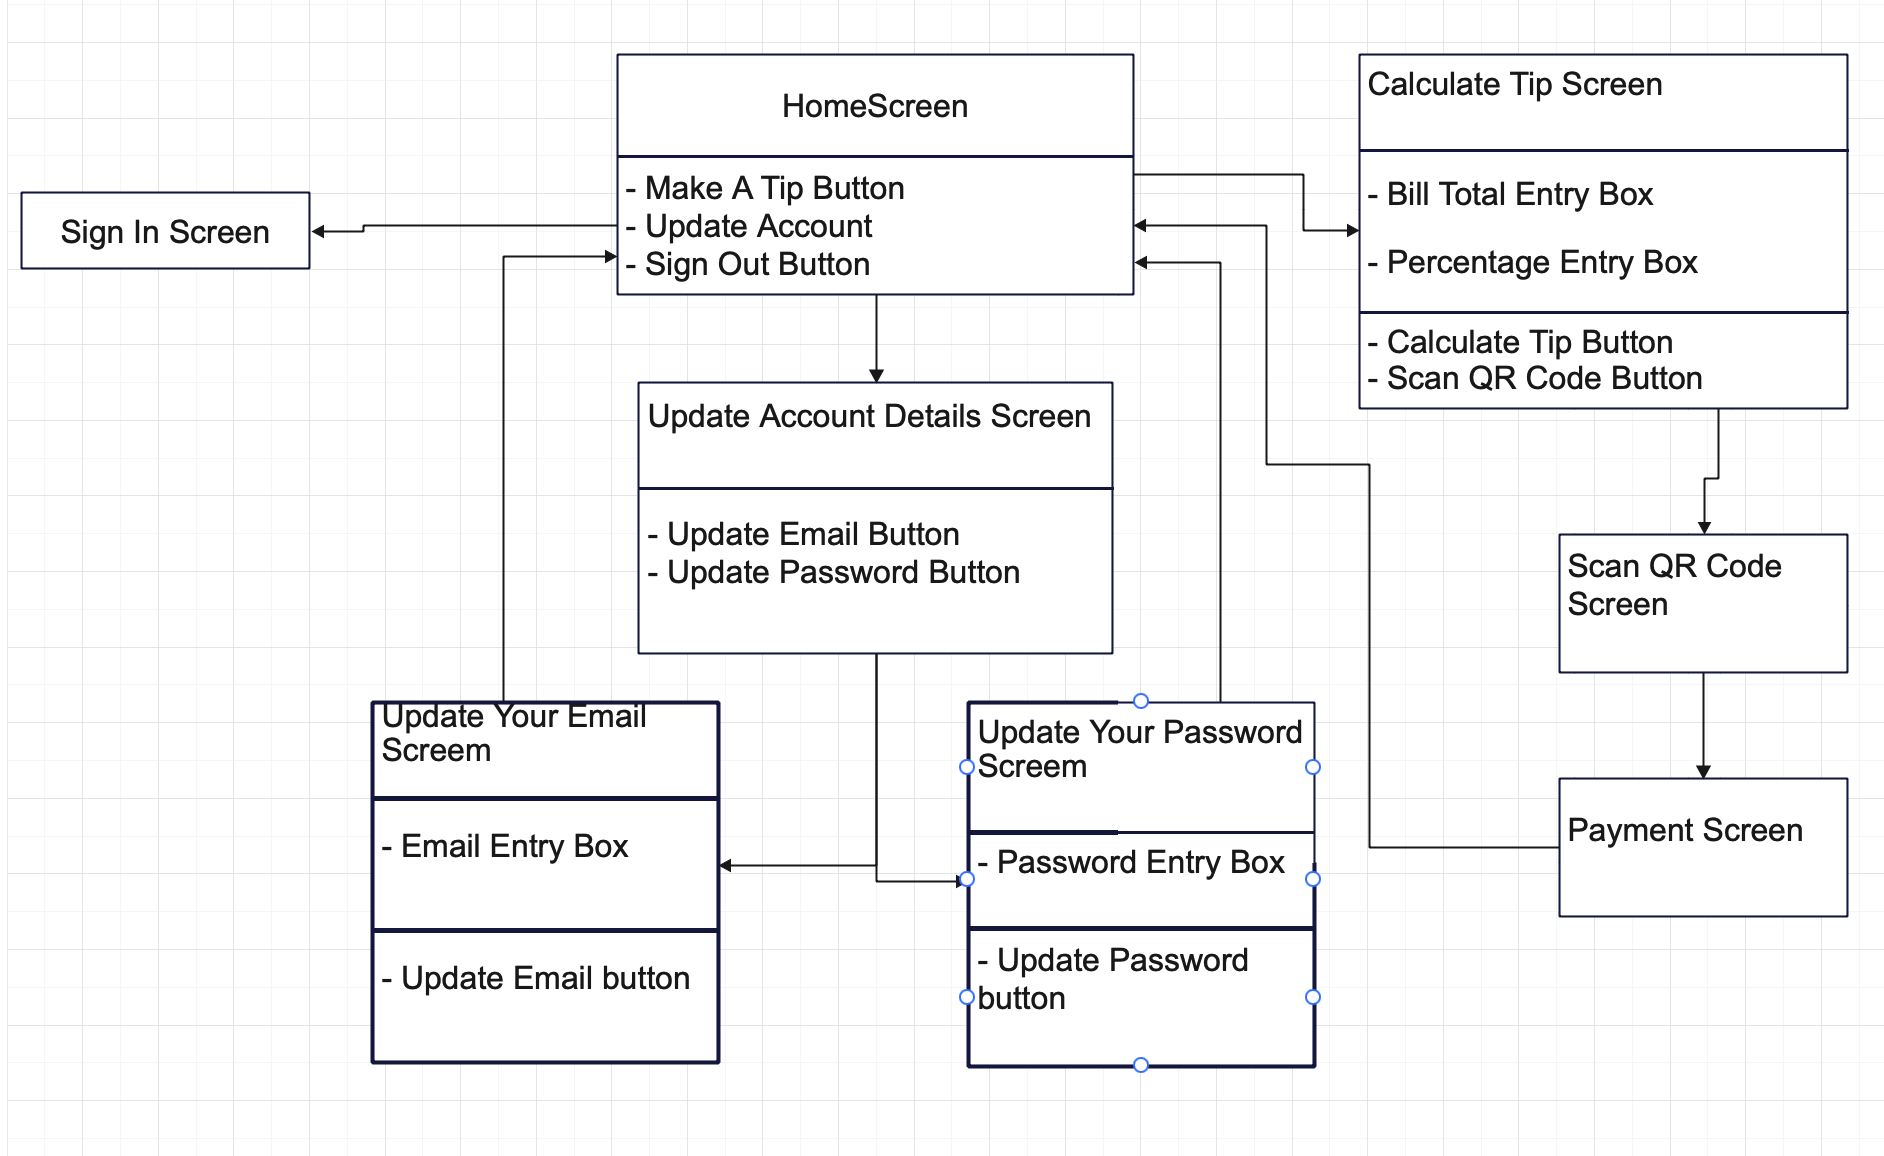
\includegraphics[scale = .40]{atu-computing-latex-template/images/HomeScreen flow.png}
\end{center}
\section{System Architecture}
The architecture is structured like this. First off, we included the MacBook in the diagram as this can depend on whether we are using a physical device or the XCode simulator. So it starts with the MacBook we developed the project on. Next it goes into Visual Studio Code. In there we used React-Native JavaScript which from there we built the application with the command 'react-native run-ios' and then if our iPhone was connected, Tipper was deployed to there or if no device was connected, it was deployed to the simulator through XCode. Next, our app interacted with AWS Amplify on the back-end to handle the login/authentication flow. Finally from the device, it uses Node to create a server that connects to Stripe via a Secret and Public Key to handle the transactions and the user is brought back to the home screen. 
\begin{center}
    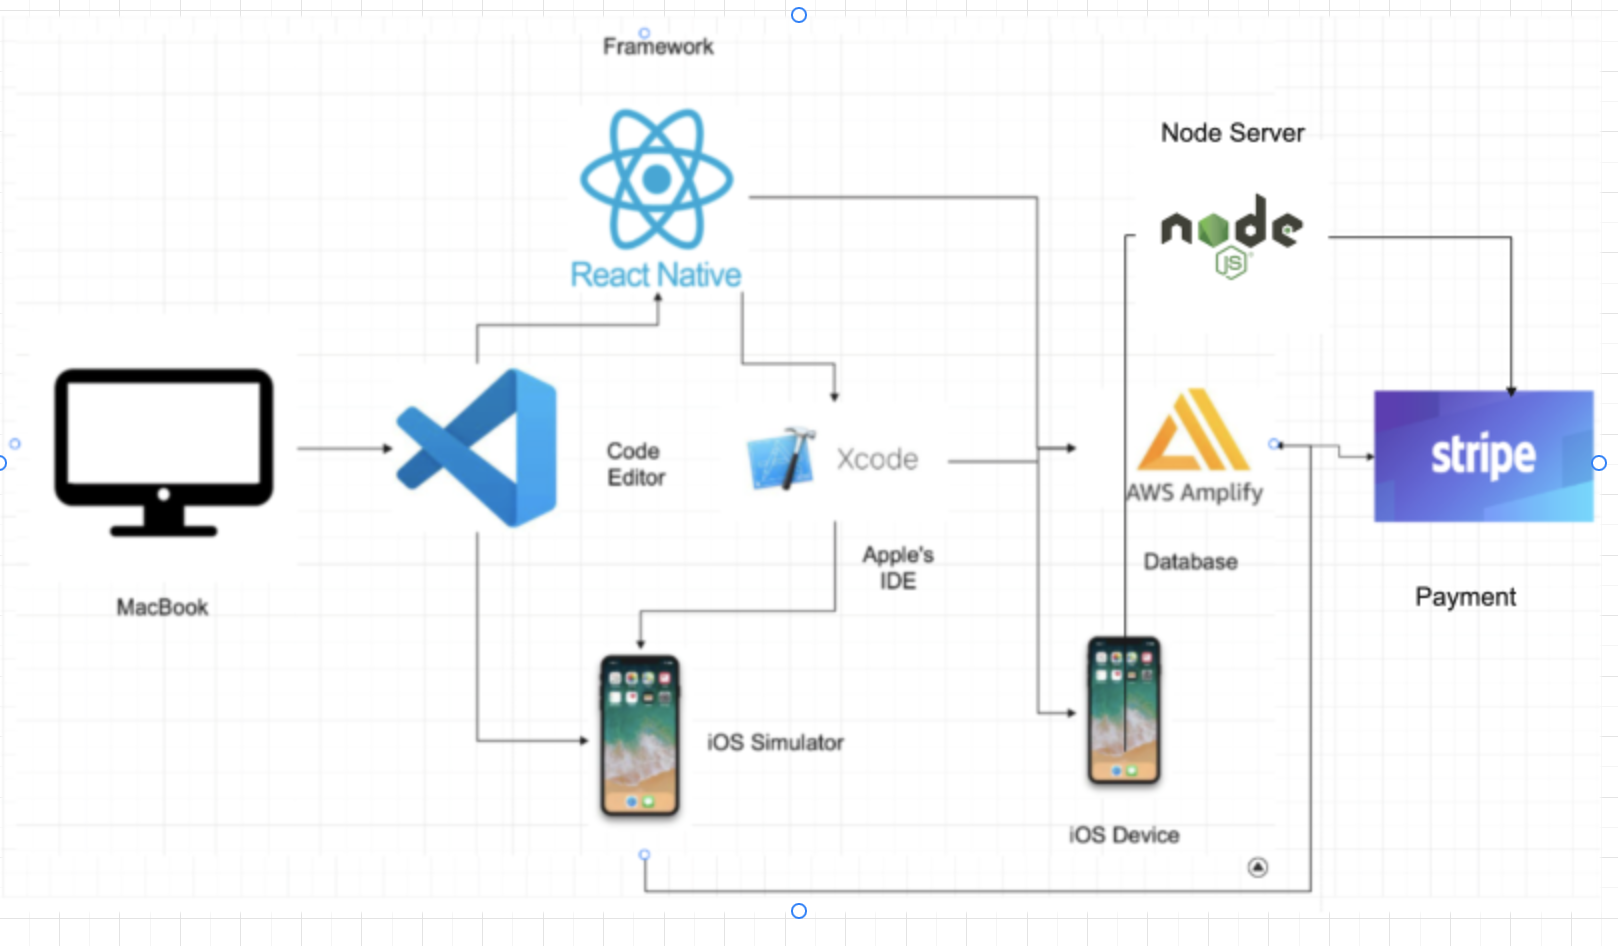
\includegraphics[scale = .55 ]{atu-computing-latex-template/images/SystemArch.png}
\end{center}


\chapter{System Evaluation}
\section{What went wrong}
Upon completion of this project, there were a few things that stood out to us during development and in the final product. To start, one thing we did not anticipate is how difficult working with packages can be. For example, a feature that we really wanted to implement was the saving of the QR code feature on the QR code generation screen. We followed the documentation, we had permissions being requested on the screen of the simulator but then nothing happened after that, the QR code never appeared in our camera roll. We assumed that maybe this was because we were using the simulator and not our device. So when we tried to build the project onto our iPhone, XCode displayed multiple errors saying as seen in the image below.
\begin{center}
    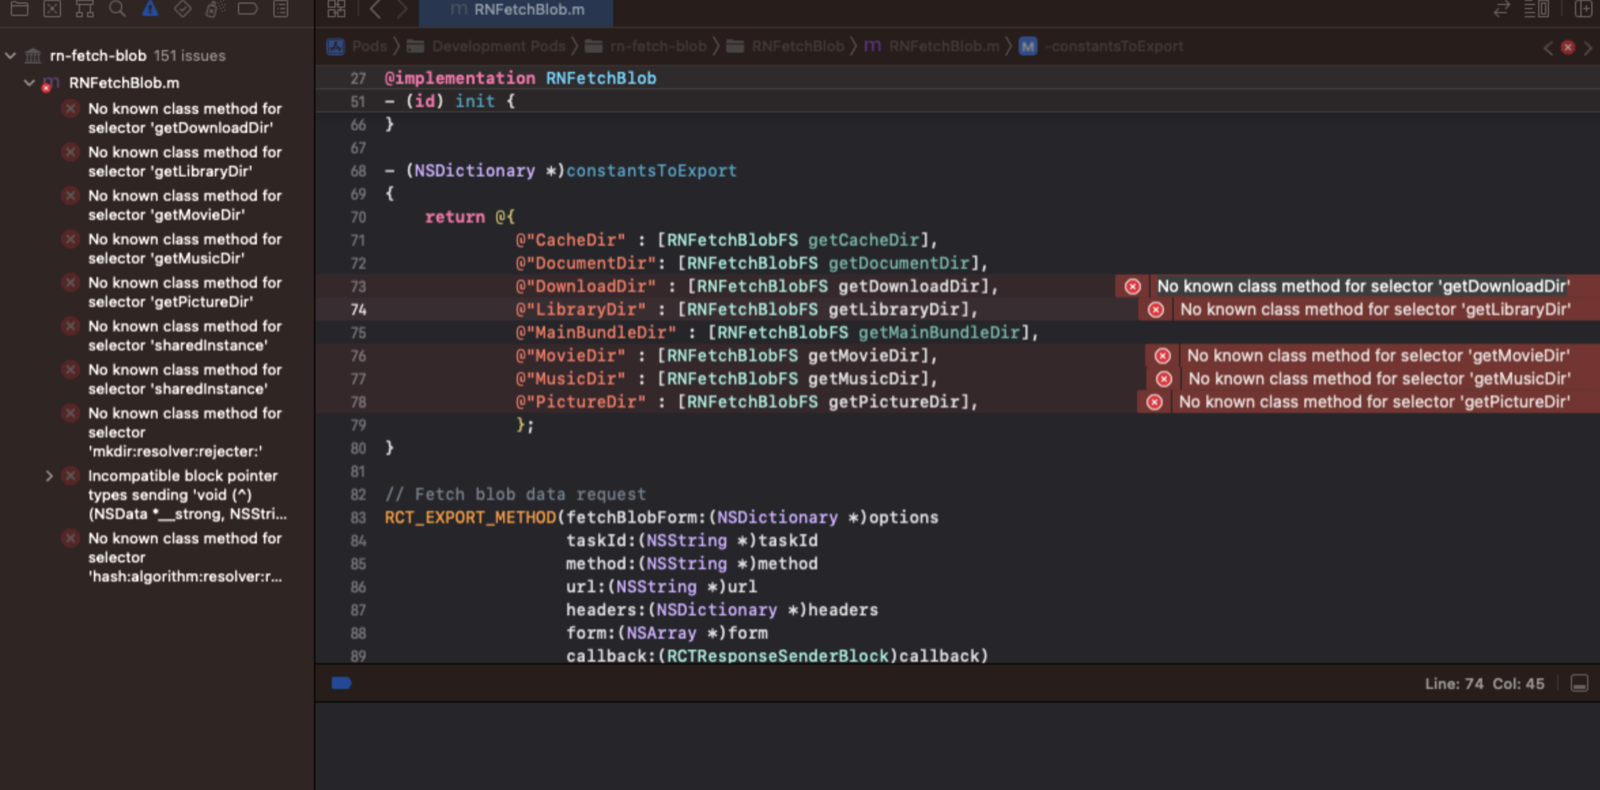
\includegraphics [scale=0.50]{atu-computing-latex-template/images/getDownloadDir.png}
\end{center}
We spent a lot of valuable time trying to implement this feature and we couldn't get it working. We were disappointed in this as we really would have liked to have that feature working. A way around this is that because the app is running on a mobile device, the user could screenshot the QR code. We were not able to find a fix to this issue and all we could find out is that the issue was due to the package 'react-native fetch-blob' that was being installed my NPM did included the methods but XCode for an unknown reason wouldn't pick up on them. Speaking XCode, something we found frustrating were the build times and the fact that we had to 'Sign Off' on every build as some modules required this but XCode would forget that we signed off every time we made a change to the project meaning we had to build our app twice, every time.

Another feature we really wanted to have was to be able to receive verification codes via SMS. AWS Amplify has this in their set of methods and we had this feature nearly working. When creating the account, the user is meant to receive a verification code. We logged this process to the console to test it and it was logging correctly with no error messages indicating to us that it was working but we never received any verification code. We tried with multiple phone numbers on different networks, checked over our configuration on AWS Amplify and everything seemed fine. In the end we settled for email verification code's. We would have preferred SMS but as long as the user can receive a code its fine.
\begin{center}
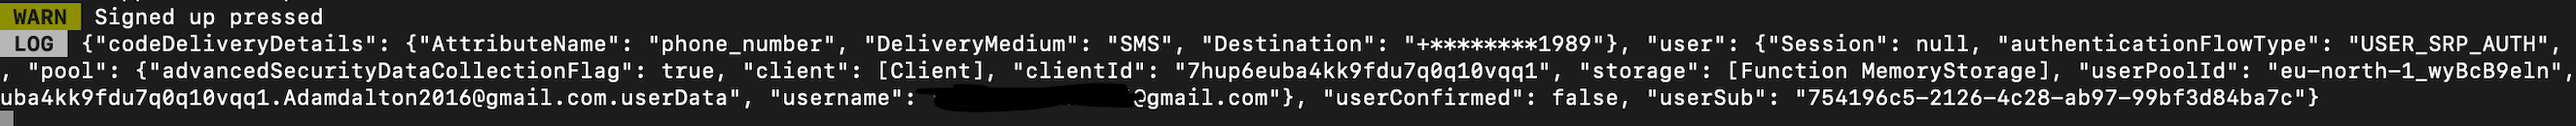
\includegraphics[scale=.30]{atu-computing-latex-template/images/codeLog.png}
\end{center}

Finally, one feature we didn't get to work fully was the user being able to reset their email address after they have signed in. The password update feature works fine but email one doesn't. We didn't get any errors when doing this to say that it didn't work, nothing in the console either. 

\section{What went well}
First off, we are happy with the features we were able to get working. The user can create an account and verify it, reset passwords, generate and scan QR codes, calculate tips etc. We for the most part completed the goal we set out to do. Secondly, from unit testing the project, we knew that the features worked individually and combining them together would work because apart from signing in, the main logic that was done was passing variables from one screen to another (e.g. the tip amount from the calculate tip screen to the QR Code scan screen) and so all we had to do was just figure out where do they fit in the overall projects structure. Overall, we are happy with the outcome of the project, especially because we had to learn a lot of new technologies to make this work.
\section{System Stability and Speed}
We can see from this table, that the build time is quite long. We tested it at 9 minutes and 4 seconds and that was from a clean build done through XCode. This included building, installing to iPhone and getting the server running. After that, any changes made required a much smaller build time. As for logging in, after entering a valid email address, was around 1.4 seconds. Opening the QR scanner was 1.5s and finally, scanning a QR code took around 1.4 seconds. 

The stability of the app is good. The only times an app crashed was when we were running the simulator and tried to open the camera which as we said is not allowed on iPhone simulators. We stress tested the app as well, running the app for a long time, going from screen to screen, entering values, closing the app and reopening. We didn't encounter any crashes when doing this on our device but as we said, crashes really only happened on the simulator.

\begin{table}[htp]
\centering
    \begin{tabular}{p{2cm}|p{2cm}|p{2cm}}
        \hline
        \multicolumn{3}{|c|}{System speed test} \\
        \hline
        Num & Test & Result \\
        \hline
        1 & Build Time & 9m 04s \\
        \hline
        2 & Change Screens & 0.87s \\
        \hline
        3 & Login Time & 1.87s \\
        \hline
        4 & Open QR & 1.5s \\
        \hline
        5 & Scan QR & 1.4s \\
        \hline
    \end{tabular}
    \caption{System speed test}
    \label{table:Stability}
\end{table}
\chapter{Conclusion}
To for this section, we will recount the purpose of the project. The goal of this application was to be able to safely and securely transfer money from one user to another by using a generated quick response code that contains a users IBAN, which is the payment destination. We wanted a user to be able to create an account, update account information, generate and scan a QR code and finally make the payment. 

The reason for developing this idea was to try and help employees of the hospitality industry, protect their wages, work and offer an alternative to the tipping culture in Ireland. We believed that if we could do that, than we would have considered this project a success. Unfortunately we could not get everything working that we would have liked to. For example the saving of the quick response code to the device was quite disappointing to say the least. We also would have liked to have given the user the option to get the verification code via text message but email was a good alternative to this. As long as the user can authenticate themselves in the sign up flow, we are happy.

We were also happy that we tried to consider expanding the application, e.g. getting the phone number from the user to potentially implement the authentication via SMS in the future. We made sure to think of scalability and accommodate for that. What we never thought of how difficult it is to actually develop a mobile application. Prior to starting the project, we knew it would be difficult to develop one, but not to this extent. It requires a lot of planning, gathering requirements, investigating technologies etc.

Even after doing all this planning, it still wasn't enough in some aspects. Take the example of MongoDB. We initially thought that would be a great option to handle the back-end but this wasn't the case. We started implementing MongoDB, read the documentation and had some features working before coming to the conclusion that it wasn't going to be a good fit for our project in the end and so was lost time and effort. We don't think this came down to poor planning but rather because this was the first time developing a mobile app like this but this leads us onto our next point.

We came at this project, having to learn nearly everything as we were developing. This isn't just limited to the React-Native framework or JavaScript. We had to learn how to use new IDE's, that being XCode and understanding its quirks and drawbacks. We had to learn how to build and deploy projects to simulators and our mobile device. Understand error messages, how to fix them and prevent them from happening again. A good example of this was 'Pods'. For a long time we didn't understand that for a lot of npm packages, we had to link them in a 'Podfile' by changing directory in the terminal into 'ios' and running the command 'pod install' and subsequently being able to link packages. Even when doing that sometimes that didn't work because of an issue with the package itself. 

Google Utilities, a software designed to help analyze, configure, optimize or maintain a computer caused issues when trying to implement a package. We had to add 'pod 'GoogleUtilities, :modular headers => true' to our podfile to get around this issue and we weren't even developing for Android but this prevented the command 'pod install' from working.

Building and running the project proved to be troublesome at times as well. As mentioned earlier, XCode often forgot that we signed off modules so sometimes we had to press build multiple times to sign off one by one. At the time this felt like frustrating but once you fix an issue once, you can do it again much faster when it came up again.

We were happy with the choice to use Stripe instead of Apple Pay. We found the dashboard on Stripe to be very informative and easy to follow. The implementation for Stripe was easy as well and gave us the opportunity to add a small server to our project using Node. The real benefit of Stripe is that it handles the security for transactions which makes our app Payment Card Industry (PCI) compliant. What this means is our app accepts, transmits, or stores the private data of cardholders is compliant with the various security measures outlined by the PCI Security Standard Council. This is done instead of trying to handle the security ourselves which to be honest, we don't think we would have been capable of implementing PCI compliance ourselves. 
\section{Outcomes}
For this, we would like to just quickly go over what came of this project
\begin{enumerate}
  \item Researched technologies and methodologies
  \item Set up the development environment
  \item Implemented the AWS Amplify Database
  \item Added Login, Authentication, Forgot Password Flow
  \item Added Home Screen with Sign out, Making a Tip and Updating Password flows
  \item Added QR Code Generation
   \item Implemented Calculating a Tip, Scanning a QR Code and Making Payment (with Stripe) flow 
   \item Building and Deploying to simulators and mobile devices
   \item Learned how to implement and debug technologies used
\end{enumerate}

\section{Final words}
To conclude, we were happy with how the project went. We went from having no idea how to develop a mobile application to investigating technologies, implementing them, bug fixing and learning how to use many new technologies and put it all together. We feel we met the purpose of the project but also achieved our own personal goal of learning how to go about this. We fully understand that there is so much more to learn about mobile application development and have probably only scratched the surface, but to know that we could apply the knowledge from this to another project is a great feeling. Yes, there were some features we couldn't get working but to know we can use what we now know as the starting point for another project is a great feeling.
\chapter{Appendencies}
This is link for our GitHub Repository https://github.com/adamdalton155/Tipper



%------------------------------------------------------------------------------------------------------	
% Generate the bibliography. You may have to build the document more than once before all of the
% references and processed and cited correctly.
% WARNING: Don't mess with any of the following unless you know what you are doing.
%------------------------------------------------------------------------------------------------------	
\bibliographystyle{unsrt}
\bibliography{references.bib}
\end{document}